\documentclass[11pt,a4paper]{article}
\usepackage[margin=2.3cm]{geometry}
\usepackage{graphicx,booktabs,amsmath,amssymb,xcolor,float,caption,tabularx}
\usepackage[hidelinks]{hyperref}
\usepackage{fancyhdr,afterpage}
\renewcommand{\topfraction}{0.9}\renewcommand{\bottomfraction}{0.8}
\renewcommand{\textfraction}{0.07}\renewcommand{\floatpagefraction}{0.85}
\setcounter{topnumber}{3}\setcounter{bottomnumber}{2}\setcounter{totalnumber}{4}
\pagestyle{fancy}\fancyhf{}
\fancyhead[L]{\small\textsc{Working draft, version 4}}
\fancyhead[R]{\small C. Alameddin, 29 Oct 2026}
\fancyfoot[C]{\thepage}
\captionsetup{font=small,labelfont=bf}
\newcommand{\dg}{^\circ}
\newcommand{\todo}[1]{\textcolor{red}{[#1]}}

\title{\textbf{Two preferred directions: a center of expansion and the plane of evil as a frame for large-scale anomalies}\\[4pt]
\large\textcolor{gray}{Working draft, version 4 --- 29 October 2026}}
\author{C. Alameddin\\ \small\texttt{calameddin@gmail.com}}
\date{}

\begin{document}
\maketitle
\thispagestyle{fancy}

\begin{abstract}
The galaxy-cluster anisotropy measured by Migkas et al.\ rejects an isotropic sky at $5\sigma$ when fitted with a center-of-expansion (CoE) geometry: treating the 71 published bins as independent, the CoE model is preferred over isotropy at $5.1\sigma$ for $A$ (the $L_X$--$T$ relation) and, with $B$ computed from the same inputs as $A$ rather than fitted separately, at $4.2\sigma$ for $B$; and its predicted two-maximum, two-minimum pattern is preferred over a plain dipole at $3.7\sigma$. With the correlations between overlapping bins taken into account, the significance against isotropy remains at least $2.6\sigma$ (Appendix~\ref{app:robust}). The geometry, a CoE seen from inside our observable sphere, was first explored to ask whether it could produce the \emph{appearance} of accelerated expansion. Turning its knobs across 229 setups (Newtonian point masses, shells and eight distributed profiles, and exact-GR LTB models, $D/R=2$--8) leaves a fixed set of features, derived in 2013--16 and later found in the Migkas data: the directional expansion peaks toward and away from the CoE with a single minimum ring between. The geometry's critical points coincide with the CMB Axis of Evil, which the author had not known of: the Migkas fit had fixed $D/R\approx3$--4.5 and a roll of $45$--$80.8\dg$, a patch covering about 1\% of possible axis directions, and the Axis of Evil lies inside it. The CoE axis and the Axis of Evil together fix a frame and a \emph{plane of evil}; tests made after the frame was fixed give a further $2.4\sigma$ for the CoE direction. The geometry predicts that the two ends of the Axis-of-Evil pattern are not antipodal but $2\theta_0\approx164\dg$ apart. In the Planck SMICA map the quadrupole--octopole axis lies $2$--$5\dg$ from the geometry's P1--P2 axis and $8$--$13\dg$ from the published axis, which places the CoE within $0.2$--$4.9\dg$ of the measured multipole plane, as predicted. The CMB alignments require a preferred plane with broken symmetry within it, and the frame supplies that plane. Seen from Earth, the best-fit CoE lies behind Orion, about $5\dg$ from Betelgeuse. These results call the strict isotropy of the cosmological principle into question, and we list tests in Planck and eROSITA data that would confirm or rule out the CoE frame.
\end{abstract}

\section{Introduction}
This work began as a question in mechanics: can a simple geometry, a point mass seen from inside an expanding sphere, produce the \emph{appearance} of accelerated expansion without the expansion actually accelerating? Working the geometry produced a short list of observables (Section~\ref{sec:origin}), derived before any of the large-scale anomalies below were compared with it.

Several were later found in independent data. The largest angular scales of the sky are not statistically isotropic. The low CMB multipoles are aligned with each other and with the dipole and equinox \cite{Schwarz04,Copi07}; several share one axis, the Axis of Evil, near $(260\dg,+60\dg)$ \cite{LM05}. The CatWISE and NVSS number-count dipoles exceed the kinematic expectation \cite{Secrest21}. Galaxy-cluster scaling relations show a direction-dependent amplitude across the sky \cite{Migkas20,Migkas21}. Raki\'c \& Schwarz \cite{RS07} showed that the CMB alignments need a preferred plane with broken symmetry within it, so one direction is not enough.

The geometry supplies two directions. The first points to a CoE beyond our observable universe. The second, set by the Axis of Evil, fixes with the CoE axis a plane we call the \emph{plane of evil}. Section~\ref{sec:model} and Appendix~\ref{app:model} give the model; Section~\ref{sec:geom} the geometry. Two non-parallel directions fix a complete orientation, so every other anomaly then has a definite place. Throughout, each result is labeled by when it entered the work: predicted before the data, identified without being built in, or tested after the frame was fixed.

\begin{figure}[!htb]\centering
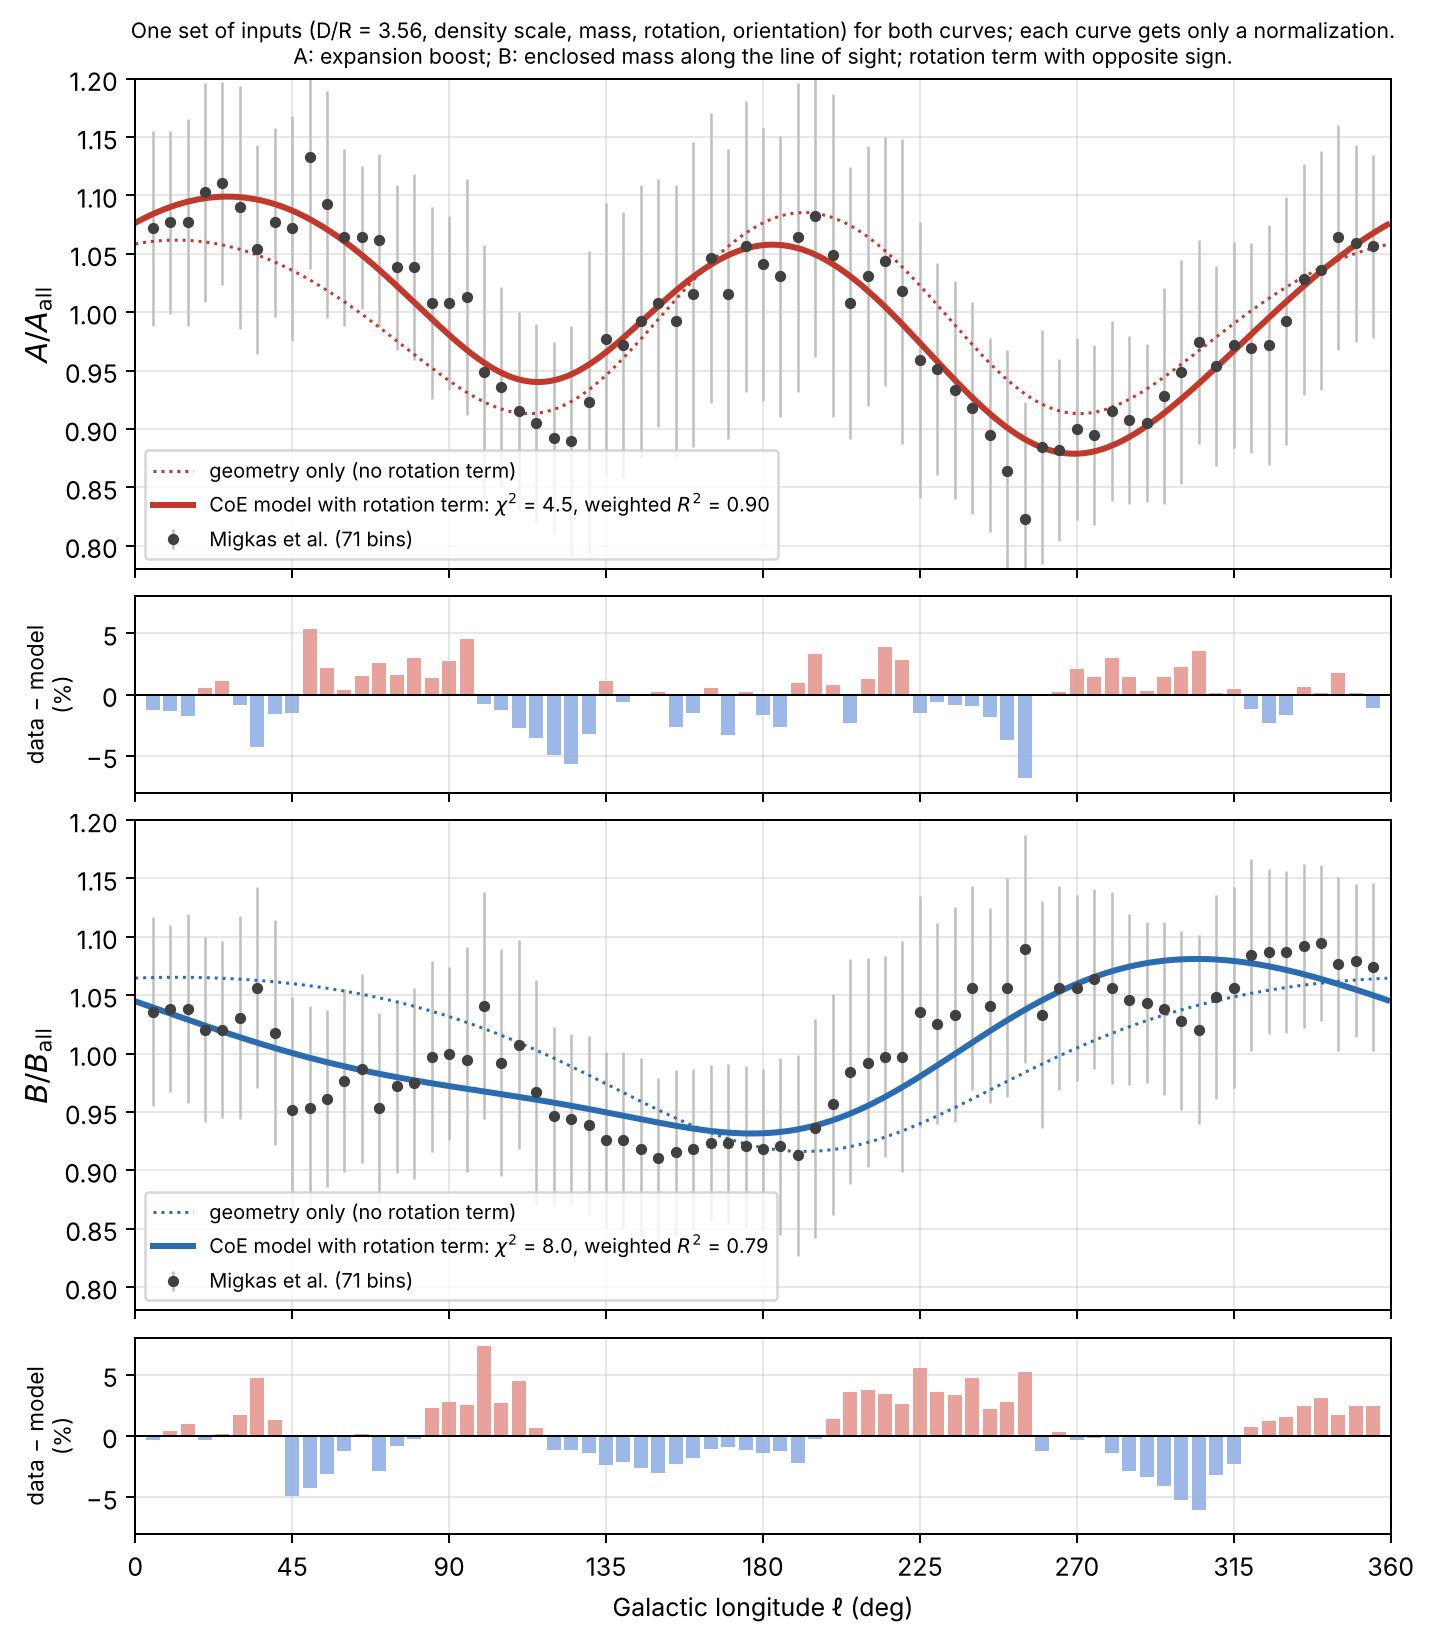
\includegraphics[width=0.82\textwidth]{figs/fig_AB.png}
\caption{Migkas $A/A_{\rm all}$ and $B/B_{\rm all}$ against Galactic longitude with the CoE model ($D/R=3.56$), and residuals. One set of inputs (density scale $L/D=0.257$, mass, rotation amplitude $a=0.180$ and phase, orientation $l_0=11.8\dg$) produces both curves (Eqs.~\ref{eq:sheetA}--\ref{eq:sheetB}); each curve gets only an offset and a scale. $A$ is the expansion boost, $B$ the enclosed mass along the line of sight; the rotation term enters with opposite signs. Dotted: geometry only (rotation term removed). $A$: $\chi^2=4.5$, weighted $R^2=0.90$; $B$: $\chi^2=8.0$, weighted $R^2=0.79$. For comparison, a plain Fourier series with five parameters fits $A$ at $R^2=0.81$.}\label{fig:AB}
\end{figure}

Figure~\ref{fig:AB} shows the observable that first confirmed the geometry: the Migkas cluster anisotropy against Galactic longitude, with the CoE model.

\section{Prior observables}\label{sec:origin}
The geometry fixes only a center of expansion at distance $D$ from the observer, who sees out to a distance $R$. It is axisymmetric about the line to the CoE, so the roll about that line is free, and the relative positions of the maximum and minimum rings follow from the geometry alone. Mass, velocity and the mass distribution were varied to understand the dynamics, not fitted to a target. The geometry constrains $D/R$ only loosely (typical setups give 3--4); the Migkas fit later preferred $D/R=3.44$, with $R^2$ nearly flat from 3 to 4.5. Table~\ref{tab:origin} (Appendix~\ref{app:origin}) lists when each observable was derived and where it was later observed; all predate Migkas et al.\ 2020 by four to seven years.


The roll is not a prior prediction: it was fitted after Migkas et al.\ 2020 appeared, to their four extrema, without any CMB input.

\section{The model}\label{sec:model}
The CoE is a mass concentration (a compact core of mass $M_c$, optionally inside a shell of density $\Omega_s=0.049$ between radii $R_{\rm in}$ and $R_{\rm out}$) at distance $D$ from the observer. Test points start on a small sphere of radius $R_s=R$ around the observer, all moving radially outward from the CoE at the start, and are integrated forward under the gravity of the enclosed mass (Newtonian, or exact general relativity in the Lemaître--Tolman--Bondi (LTB) solution). The directional expansion seen by the observer at angle $\theta$ from the anti-CoE direction is
\begin{equation}
a_f(\theta)=\frac{\lvert\mathbf v(\theta)-\mathbf v_{\rm obs}\rvert}{\lvert\mathbf x(\theta)-\mathbf x_{\rm obs}\rvert},\qquad H(\theta)\propto\sqrt{A(\theta)},
\end{equation}
normalized to its mean over directions. Placed on the sky with the CoE at Galactic longitude $l_0+180\dg$, it is compared with Migkas's normalized scaling-relation amplitude (the $L_X$--$T$ normalization $A/A_{\rm all}$, and the second relation $B/B_{\rm all}$, each relative to its all-sky value) as
\begin{equation}
A_{\rm model}(l)=s\,\bigl[1-a\sin(l+\phi)\bigr]\,a_f(l-l_0).
\end{equation}
The fitted parameters are $M_c/M_{\rm crit}(D)$, $R_{\rm in}$, $R_{\rm out}$, $l_0$, $a$, $\phi$ and the normalization $s$ (seven in all; $D/R$ is held fixed). Appendix~\ref{app:model} gives the integration details; the derivation follows the author's earlier letter.

\paragraph{One set of inputs for $A$ and $B$.} The author's original one-step formulation gives both curves from the same inputs. For a point P on the observable sphere at angle $\theta$ (observer at distance $D$ from the CoE), the CoE--P distance and the mass inside it, for an exponential density of scale $L$, are
\begin{equation}
r=\sqrt{(D+R\cos\theta)^2+R^2\sin^2\theta},\qquad m(<r)=M_{\rm tot}\Bigl[1-e^{-r/L}\Bigl(1+\frac rL+\frac{r^2}{2L^2}\Bigr)\Bigr],
\end{equation}
with $M_{\rm tot}$ set so that $m(<D)=M$. With Hubble-like flow $\mathbf v=k\mathbf r$ and gravity $\mathbf a=-Gm(<r)\hat{\mathbf r}/r^2$, the velocity relative to the observer after one step $\Delta t$ gives
\begin{align}
A(\theta)&=\bigl[1-a\sin(\theta+\phi)\bigr]\,\frac{\lvert\Delta\mathbf v+\Delta\mathbf a\,\Delta t\rvert}{kR},\label{eq:sheetA}\\
B(\theta)&=\bigl[1+a\sin(\theta+\phi)\bigr]\,\frac{m(<r)}{M}.\label{eq:sheetB}
\end{align}
$A$ is the expansion boost from the CoE's gravity; $B$ is the relative mass between the CoE and P in that direction. The rotation term has the same amplitude and phase in both, with opposite sign. Once $D/R$, $L/D$, $M$, $a$, $\phi$ and the orientation $l_0$ are chosen, \emph{both} curves are fixed; only an offset and a scale are fitted per curve. $B$ is therefore not an independent fit: tuning the inputs on $A$ alone leaves the mass profile unconstrained and spoils $B$, and it is $B$ that pins the density scale.

\paragraph{The rotation term is a second direction.} The orientation ($l_0$ and the roll about the CoE axis) places the axisymmetric pattern on the sky. The term $1\pm a\sin(\theta+\phi)$ does something no orientation of an axisymmetric pattern can: it adds a dipole across the sky that does not point along the CoE axis. If it were a free knob, its direction would be arbitrary. Profiling the joint fit over the phase, with all other inputs refitted, puts the direction in which $A$ is boosted most (and $B$ least) at Galactic longitude $l=73\dg\pm14\dg$ ($1\sigma$; $44$--$100\dg$ at $2\sigma$). This is $7\dg$ from the longitude of the Axis of Evil at its P1 end, $(80\dg,-60\dg)$, and $7\dg$ from that of the P1--P2 axis, $(65.7\dg,-56.9\dg)$; the Axis of Evil was not used in the fit. An arbitrary direction falls this close about 10--15\% of the time, so this supports the reading of the term as the frame's second direction rather than adding a separate significance. The 1-D curve constrains only longitude and cannot separate the two axes. A sharper test fixes $a$ and $\phi$ from the frame and refits $A$ and $B$ with them held fixed.

\section{Geometry}\label{sec:geom}
The observer sits at the center of an observable sphere of radius $R$; the CoE lies a distance $D$ away. Points on the sphere at the same distance $D$ from the CoE as the observer lie on a circle at angle $\theta_0$ from the CoE direction,
\begin{equation}
\cos\theta_0=\frac{R}{2D}.
\end{equation}
The circle of radius $D$ about the CoE passes through the observer and crosses the sphere at two critical points, P1 and P2 (Fig.~\ref{fig:frame}). The plane through the CoE axis, P1 and P2 is the plane of evil. In the geometry the CMB multipole plane is the plane normal to the P1--P2 axis: because P1 and P2 sit at the same angle $\theta_0$ on either side of the CoE axis, that axis is exactly perpendicular to the CoE direction for every $D/R$, so the multipole plane contains the CoE and crosses the plane of evil at right angles. $D/R$ came from the Migkas fit ($3.44$, broad from 3 to 4.5). The Axis of Evil was then found at the critical-point structure: it is the axis through P1 and its antipode, the headless axis produced by the arc from P1 to P2 on the circle about the CoE through the observer. Taking P1 exactly on the published axis gives $D/R=3.56$ and roll $60.18\dg$ (Table~\ref{tab:geom}), inside the range the Migkas fit already allowed. The P1--P2 axis is then $(245.7\dg,+56.9\dg)$, $90.0\dg$ from the CoE and $8.1\dg$ from the published headless axis. The plane normal to the published axis misses the CoE by $8.1\dg$; the plane normal to the P1--P2 axis contains it.

\paragraph{The ends of the axis are not antipodal.} Published Axis-of-Evil directions are headless axes: each fit assumes the two ends of the pattern lie exactly $180\dg$ apart. In the geometry the two ends are P1 and P2, which lie on either side of the CoE axis at $\theta_0$ from it, so their separation is
\begin{equation}
\Delta=2\theta_0=2\arccos\!\left(\frac{R}{2D}\right)\approx164\dg\quad(D/R=3.56).
\end{equation}
The P1--P2 direction is exactly perpendicular to the CoE axis for every $D/R$, and both ends lean $90\dg-\theta_0=\arcsin(R/2D)\approx8\dg$ toward the CoE side. A headless fit forced onto such a pattern returns an axis between the two ends, which would contribute to the scatter among published axes and to the imperfect quadrupole--octopole alignment. Measuring the two ends separately gives $D/R$ directly from the CMB (Section~\ref{sec:concl}).

\begin{table}[!htb]\centering\small
\caption{Inputs and derived quantities of the frame.}\label{tab:geom}
\begin{tabularx}{\textwidth}{>{\raggedright\arraybackslash}p{3.6cm}X>{\raggedright\arraybackslash}p{2.6cm}}\toprule
Quantity & Value & Role\\\midrule
CoE direction $(l,b)$ & $(180\dg,-15\dg)$ & input\\
Axis of Evil & $(260\dg,+60\dg)\leftrightarrow(80\dg,-60\dg)$ & input \cite{LM05}\\
$\theta_0$ & $81.94\dg$ & derived\\
$D/R$ & 3.44 Migkas fit (3--4.5); 3.564 with P1 on the Axis of Evil ($D=51.0$ Gpc) & fit; then derived\\
Roll about CoE axis & $60.18\dg$ (alternative $240.18\dg$); Migkas window $45$--$80.8\dg$ & derived\\
P2 & $(234\dg,+52.5\dg)\leftrightarrow(54\dg,-52.5\dg)$ & derived\\
P1--P2 separation & $2\theta_0=163.9\dg$ (not $180\dg$) & derived\\
P1--P2 axis (multipole-plane normal) & $(245.7\dg,+56.9\dg)$, $90.0\dg$ from the CoE & derived\\
Plane-of-evil normal & $(98.4\dg,+28.7\dg)$ & derived\\\bottomrule
\end{tabularx}
\end{table}

\begin{figure}[!htb]\centering
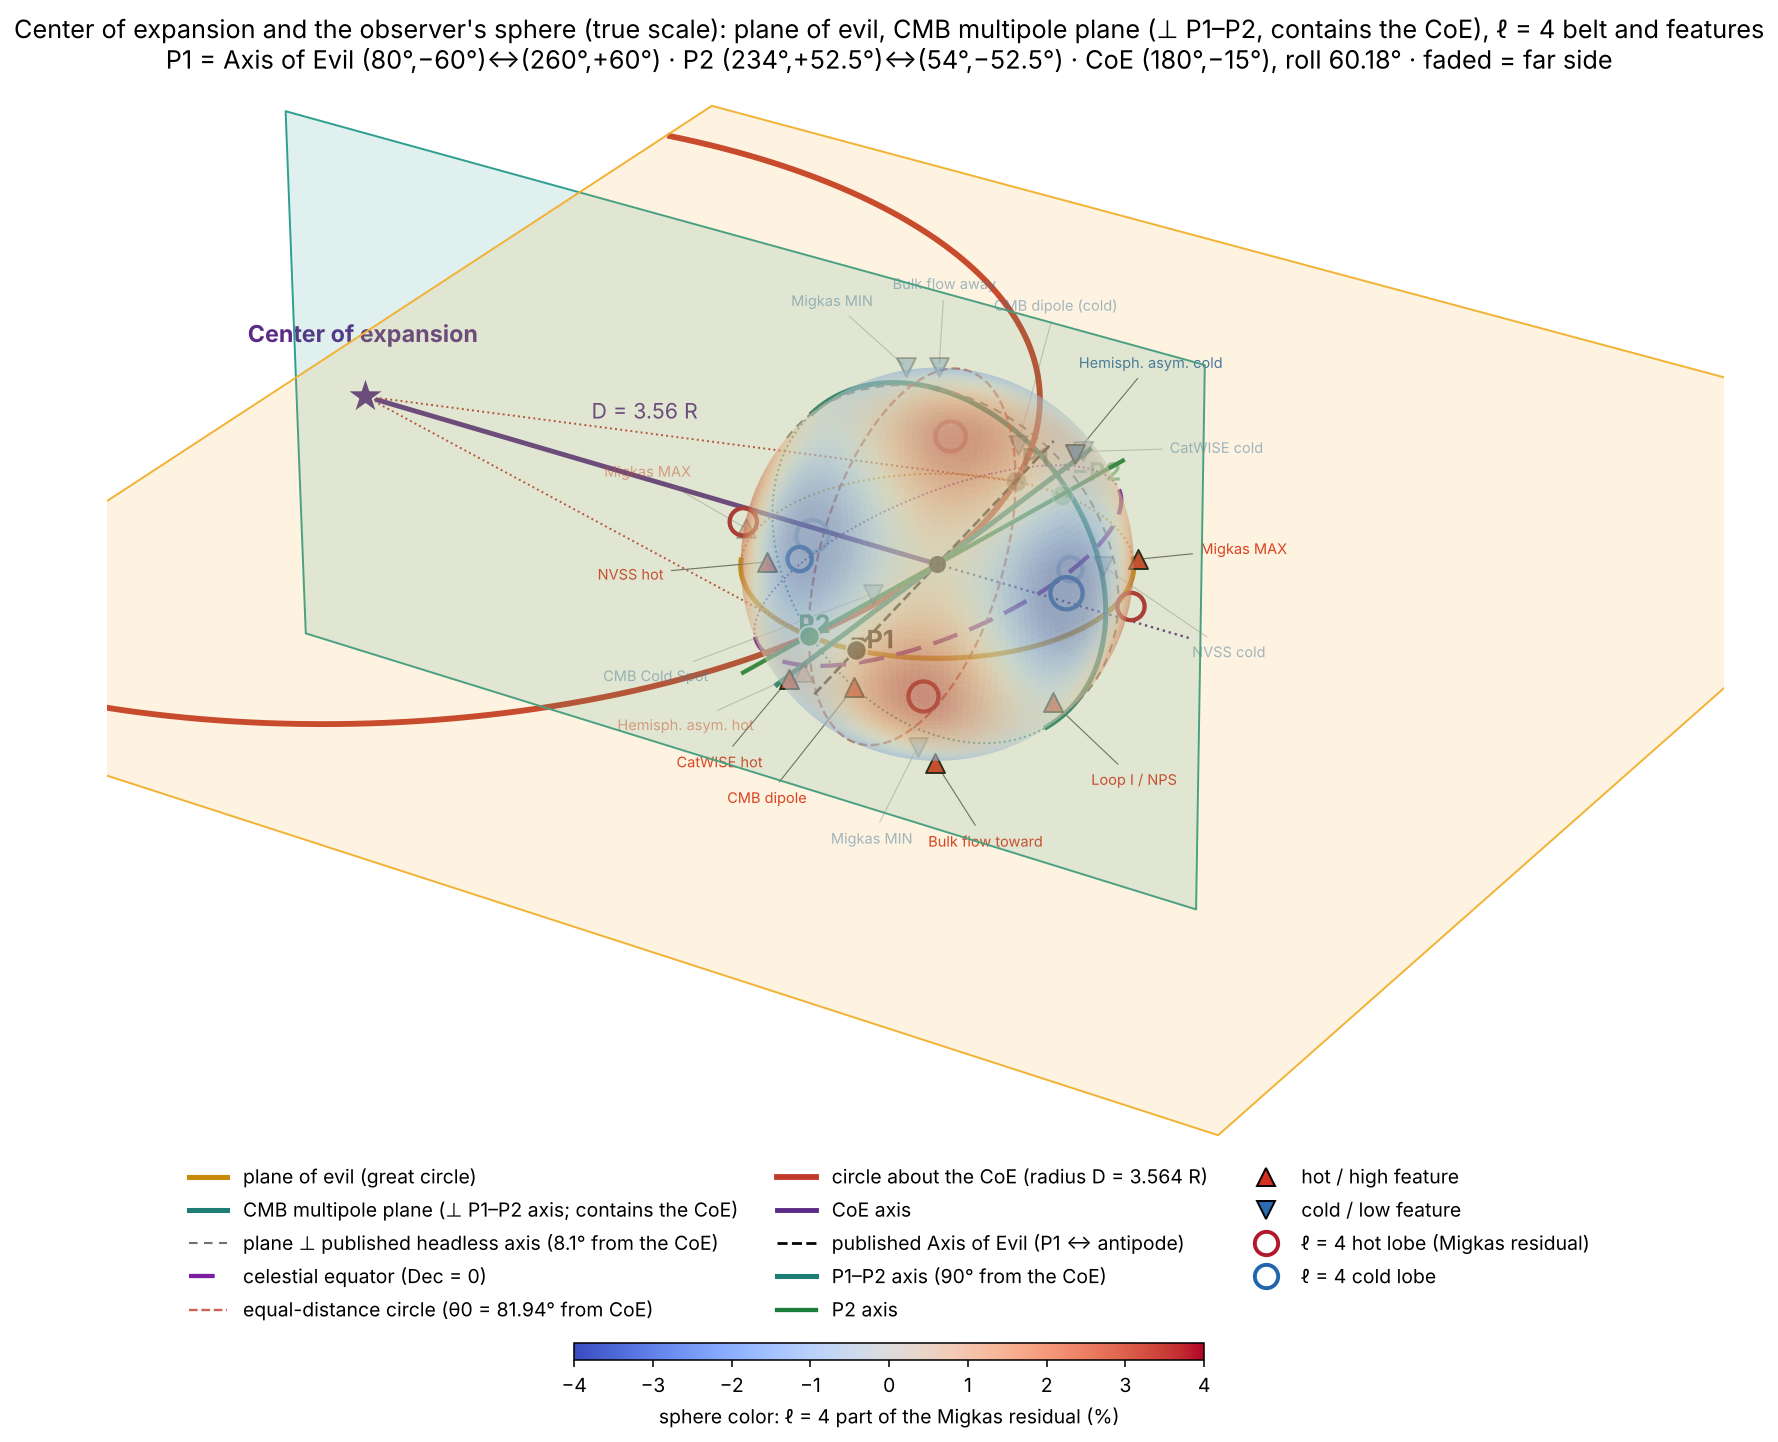
\includegraphics[width=\textwidth]{figs/fig1_frame3d_coe_p1p2.png}
\caption{The center of expansion and the observer's sphere, to scale ($D=3.56R$). Gold: plane of evil; teal: CMB multipole plane, normal to the P1--P2 axis, which contains the CoE and its axis and crosses the plane of evil at right angles; gray dashed: plane normal to the published headless Axis of Evil, $8.1\dg$ from the CoE; purple dashed: celestial equator. The sphere is colored by the $\ell=4$ part of the Migkas residual (Sec.~\ref{sec:fit}). Triangles: anomaly features (red hot/high, blue cold/low); faded symbols are on the far side. Two edge-on views are in Appendix~\ref{app:views}.}\label{fig:frame}
\end{figure}

\section{What survives turning the knobs}\label{sec:knobs}
To separate what the geometry predicts from what depends on its settings, we computed the directional expansion $A(\theta)$, with $\theta$ measured from the anti-CoE direction, in 229 valid setups. These were Newtonian point mass + shell (28), eight distributed density profiles (180: exponential cores of three widths, power law, Gaussian, cored, inner shell, Sedov--Taylor blast), and exact-GR LTB point mass + shell (21), each over $D/R=2$--8 with varied masses and backgrounds. Setups in which matter falls back or shells cross were discarded as unphysical. The Hubble rate follows $H\propto\sqrt{A}$, so it shares the same extrema.

\begin{table}[!htb]\centering\small
\caption{Which observables hold across setups.}\label{tab:knobs}
\begin{tabularx}{\textwidth}{>{\raggedright\arraybackslash}p{5.2cm}>{\raggedright\arraybackslash}X>{\raggedright\arraybackslash}p{2.5cm}>{\raggedright\arraybackslash}p{2.3cm}}\toprule
Observable & Newtonian (208) / LTB (21) & Robust? & Observed\\\midrule
$A$: maxima at both poles, one minimum ring & 208/208 / 20/21 & yes & yes\\
Minimum ring on the equal-distance circle & Newtonian: $0.4$--$8.5\dg$ outside it (mean $3.8\dg$), set by $D/R$ alone; LTB: $97.5$--$100.5\dg$ from anti-CoE & yes & Migkas minima at $97\dg$, $104.5\dg$\\
Two maxima + two minima along any great circle through the CoE axis & follows from row 1 & yes & Migkas 1-D curve\\
Global maximum on the CoE side & 180/208 / 18/21 (flips for very extended or very light cores) & mostly & yes\\
Density does not rise away from the CoE & 208/208 (falls, or flat inside a uniform shell) & yes & sign only: CatWISE excess dipole\\
Critical points P1, P2 and their plane & pure geometry, any $D/R>0.5$ & yes & Axis of Evil\\
Value of $D/R$ & set by the configuration & no (fitted) & 3.44 (Migkas); 3.56 (Axis of Evil)\\\bottomrule
\end{tabularx}
\end{table}

Allowing the CoE inside or near our sphere changes the pattern (160 further runs, $D/R=0.55$--1.9). For $D/R\lesssim0.85$, $A$ becomes a simple dipole, maximum away from the CoE and minimum toward it, with no ring; between 0.85 and 1.3 the shape is transitional; from 1.6 upward the minimum ring returns. The observed two-maximum, two-minimum structure therefore requires the CoE to lie outside the observable sphere, and disfavors a center inside it such as that of \cite{Bao23}.

In the Newtonian setups the minimum ring of $A$ lies on or just outside the circle of the critical points ($0.4$--$8.5\dg$ outside), and its position depends only on $D/R$, not on the mass or profile (Fig.~\ref{fig:knobs}). In exact GR the minimum stays near $97.5$--$100.5\dg$ from the anti-CoE for every $D/R$ from 2 to 8, while the circle moves from $104.5\dg$ to $93.6\dg$; the link is therefore close at $D/R\approx3$--4 but not exact in general. The geometry therefore ties the cluster-anisotropy minimum to the same circle that holds the Axis of Evil. With the data-fitted CoE $(198\dg,-4\dg)$, the two Migkas minima lie $97.0\dg$ and $104.5\dg$ from the anti-CoE and the Axis of Evil $100.0\dg$, all on the predicted ring. That CoE direction was itself fitted to the Migkas map, so this agreement is partly built in; the ring's existence and its link to the critical circle are not.

\begin{figure}[!htb]\centering
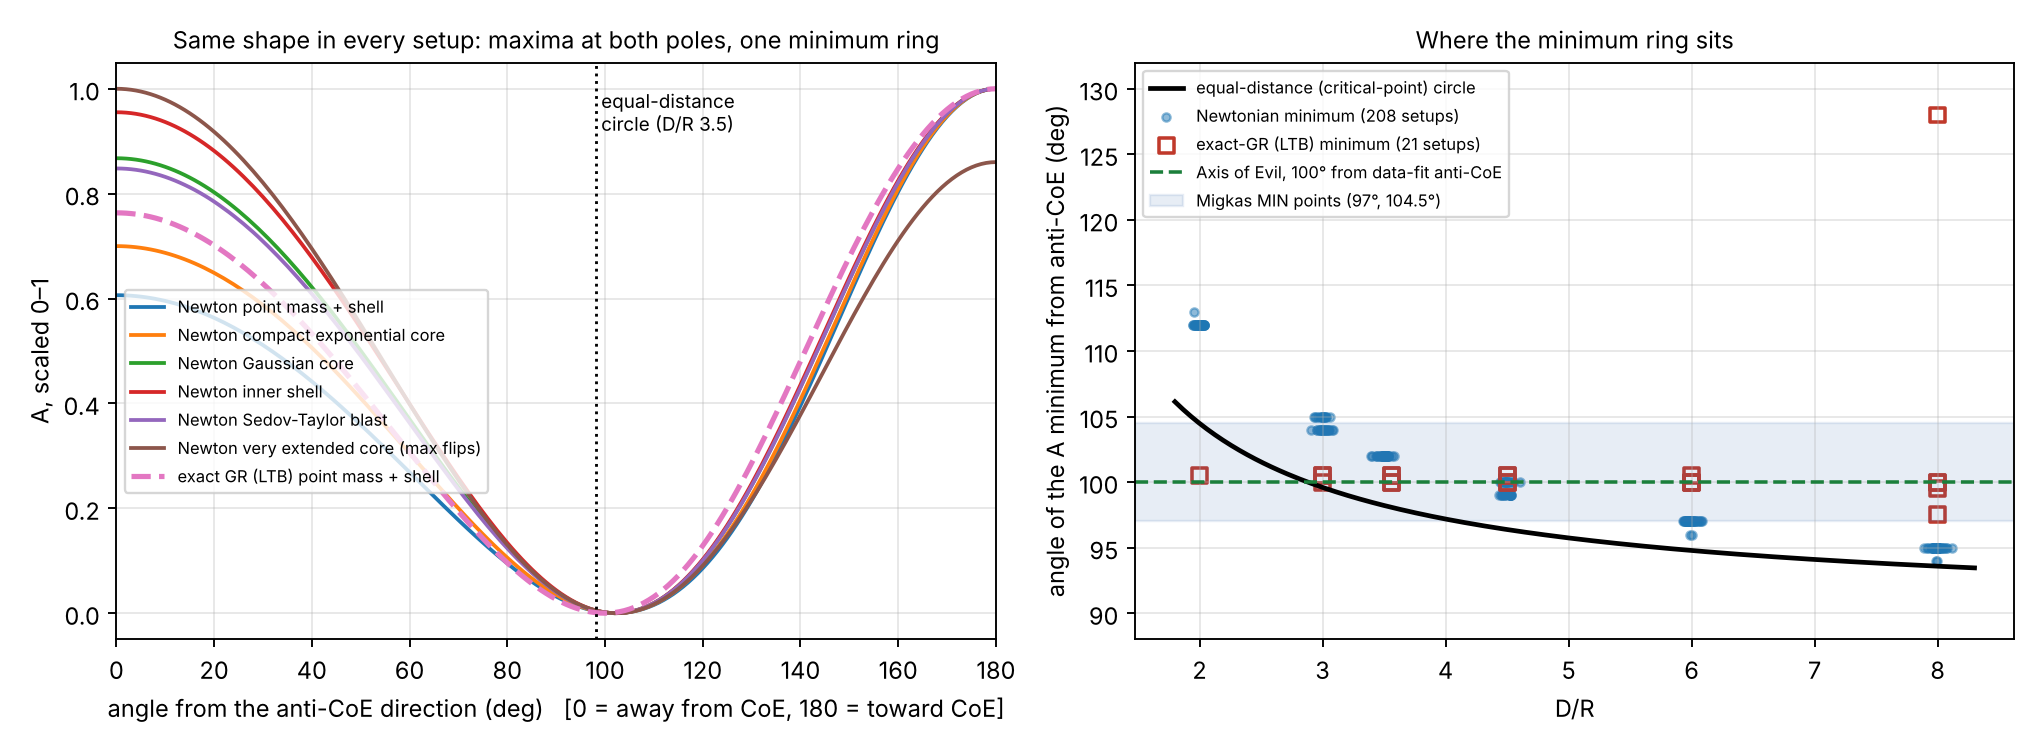
\includegraphics[width=\textwidth]{figs/fig_knobs.png}
\caption{Left: $A(\theta)$ in representative setups, scaled 0--1; every setup has maxima at both poles and one minimum ring. Right: angle of the minimum against $D/R$ for all setups, with the equal-distance circle, the Axis of Evil and the Migkas minima.}\label{fig:knobs}
\end{figure}

\section{Data}
\begin{itemize}\setlength\itemsep{1pt}
\item \textbf{Migkas et al.\ cluster anisotropy} \cite{Migkas20,Migkas21}: the 2-D $A/A_{\rm all}$ map from $75\dg$ cones over 313 clusters with its pixel covariance, and the 1-D $A(l)$ curve (71 points).
\item \textbf{Anomaly catalog} (12 features, Table~\ref{tab:features}): CMB dipole and its cold pole, CMB Cold Spot, bulk flow toward/away, NVSS and CatWISE dipoles (both ends) \cite{Secrest21}, hemispherical asymmetry (both ends), Loop~I/NPS. Loop~I is a Galactic foreground and is included as a control direction. CMB features are compared with the $A$ residual and source-count features with the $B$ residual, as fixed before scoring.
\item \textbf{Pantheon+ supernovae} \cite{Scolnic22}: Hubble-residual dipole and quadrupole (Section~\ref{sec:sym}).
\end{itemize}

\section{Fitting the cluster anisotropy}\label{sec:fit}
The CoE model fits the Migkas 1-D curves (Fig.~\ref{fig:AB}). A ring model in the frame reproduces the Migkas 2-D map at $r=0.79$. It wraps the Migkas $A(\theta)$ curve on rings about the anti-CoE direction, blends the two halves of each ring, and blends neighboring rings with a Gaussian of width $\sigma$ (Fig.~\ref{fig:blends}): $r=0.59$ without cross-ring blending, 0.70 at $\sigma=30\dg$, 0.77 at $50\dg$, 0.79 with finer rings at $20\dg$.

With the CoE axis fixed, the 2-D map gives its best match at a roll of $50\dg$ for every blend width from $0\dg$ to $90\dg$ (Fig.~\ref{fig:roll}). The Axis of Evil fixes the roll at $60.18\dg$, within 0.006 of the maximum match.

The map minus the model leaves 3.5\% rms (Fig.~\ref{fig:chain}). Its $\ell=4$ part carries $2.5\times$ the noise power ($p=0.016$ from 1000 simulations of the map covariance) and is the only multipole above noise (Fig.~\ref{fig:multipoles}). The model contributes 0.04\% rms at $\ell=4$, so the belt is in the cluster data. Its eight strongest lobes lie $12$--$22\dg$ from the plane of evil and alternate hot and cold around it. The $A(\theta)$ curve comes from the same clusters as the map, so $r$ overstates independent agreement; the roll and the $\ell=4$ orientation are not set by the curve.



\begin{figure}[!htb]\centering
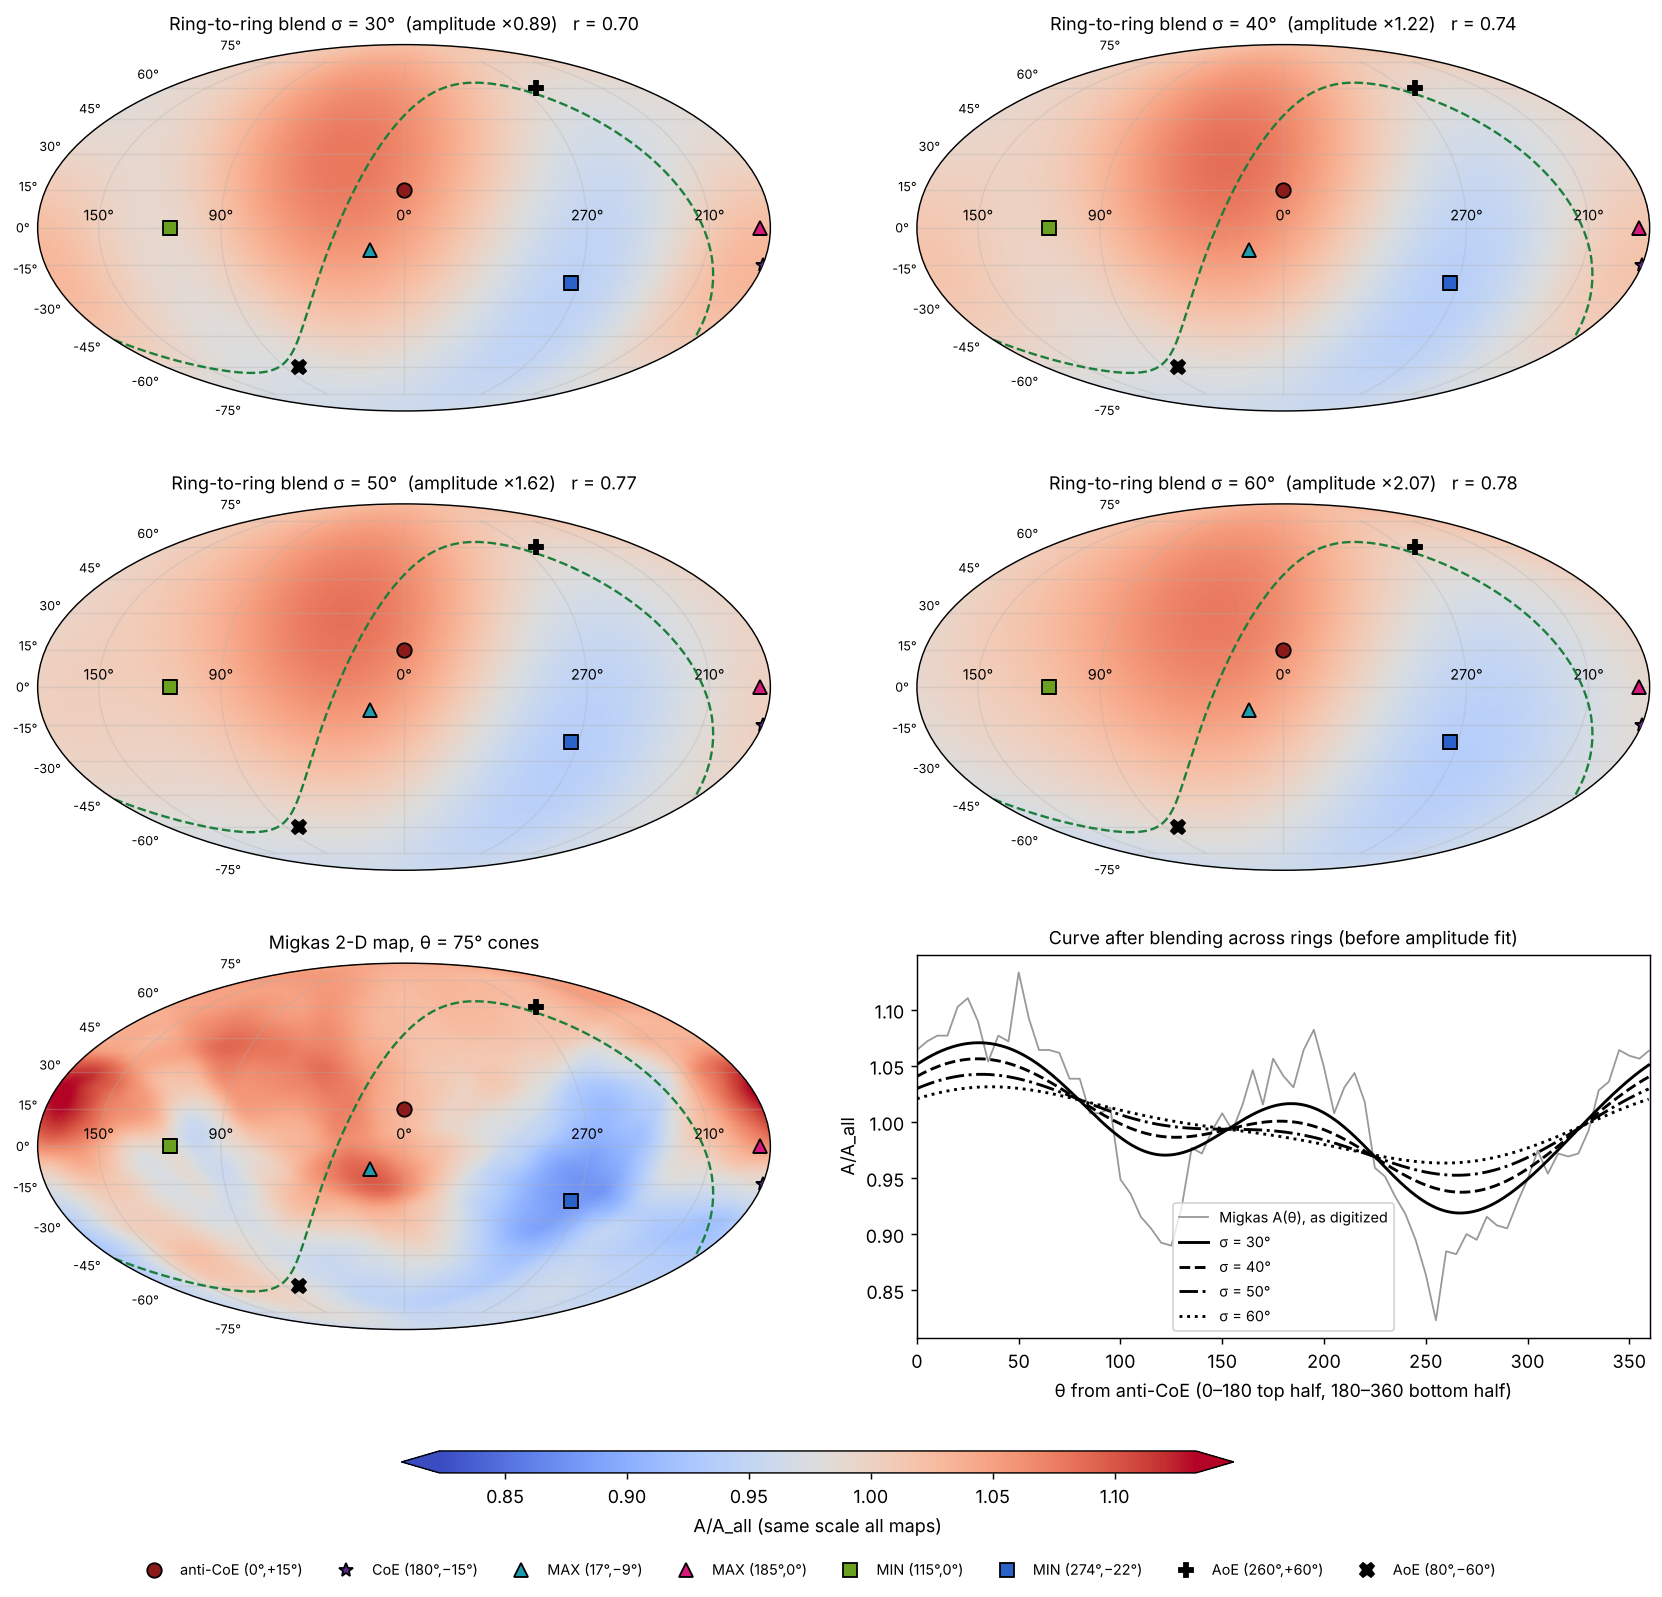
\includegraphics[width=0.9\textwidth]{figs/fig3_ringblends.png}
\caption{Ring-to-ring blends of width $\sigma=30$--$60\dg$ at the Axis-of-Evil roll, against the Migkas 2-D map (bottom left). Bottom right: the $A(\theta)$ curve before and after blending.}\label{fig:blends}
\end{figure}

\begin{figure}[!htb]\centering
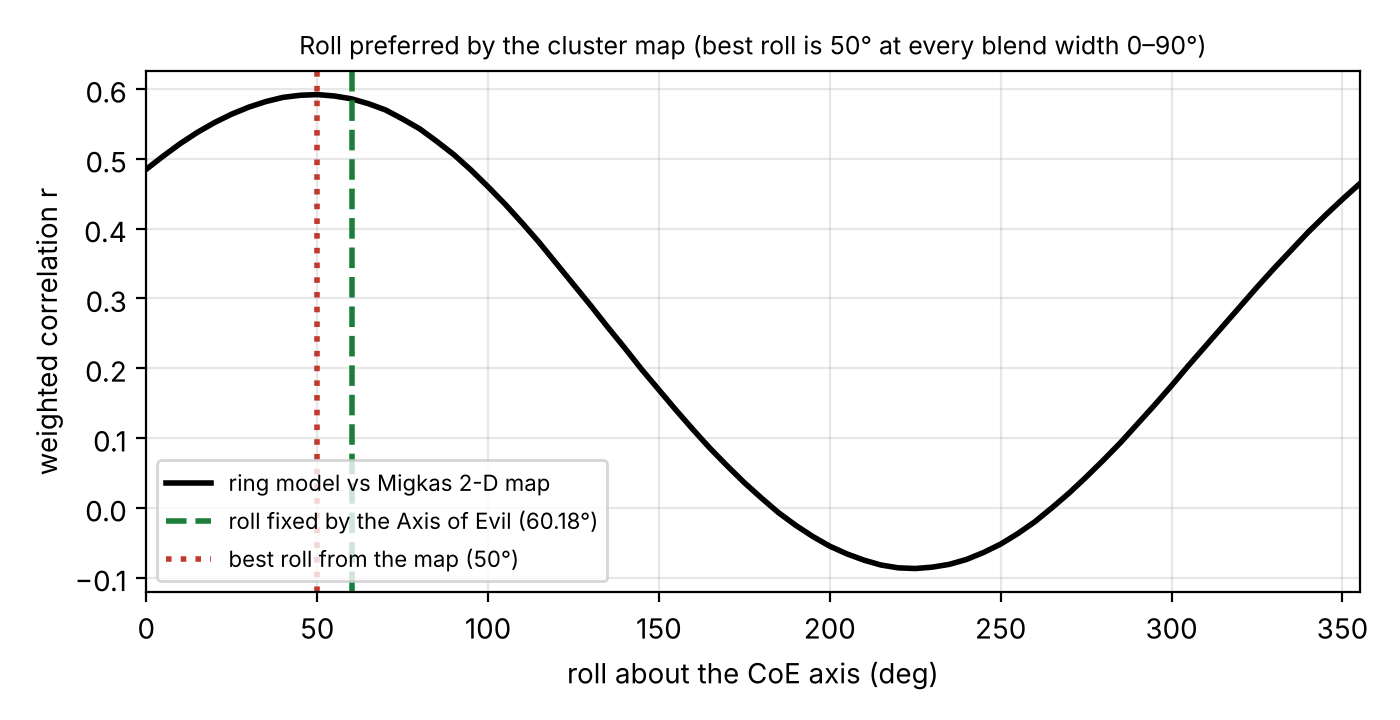
\includegraphics[width=0.72\textwidth]{figs/fig2_roll.png}
\caption{Match between the ring model and the Migkas 2-D map as the roll varies. The map prefers $50\dg$; the Axis of Evil fixes $60.18\dg$.}\label{fig:roll}
\end{figure}

\begin{figure}[!htb]\centering
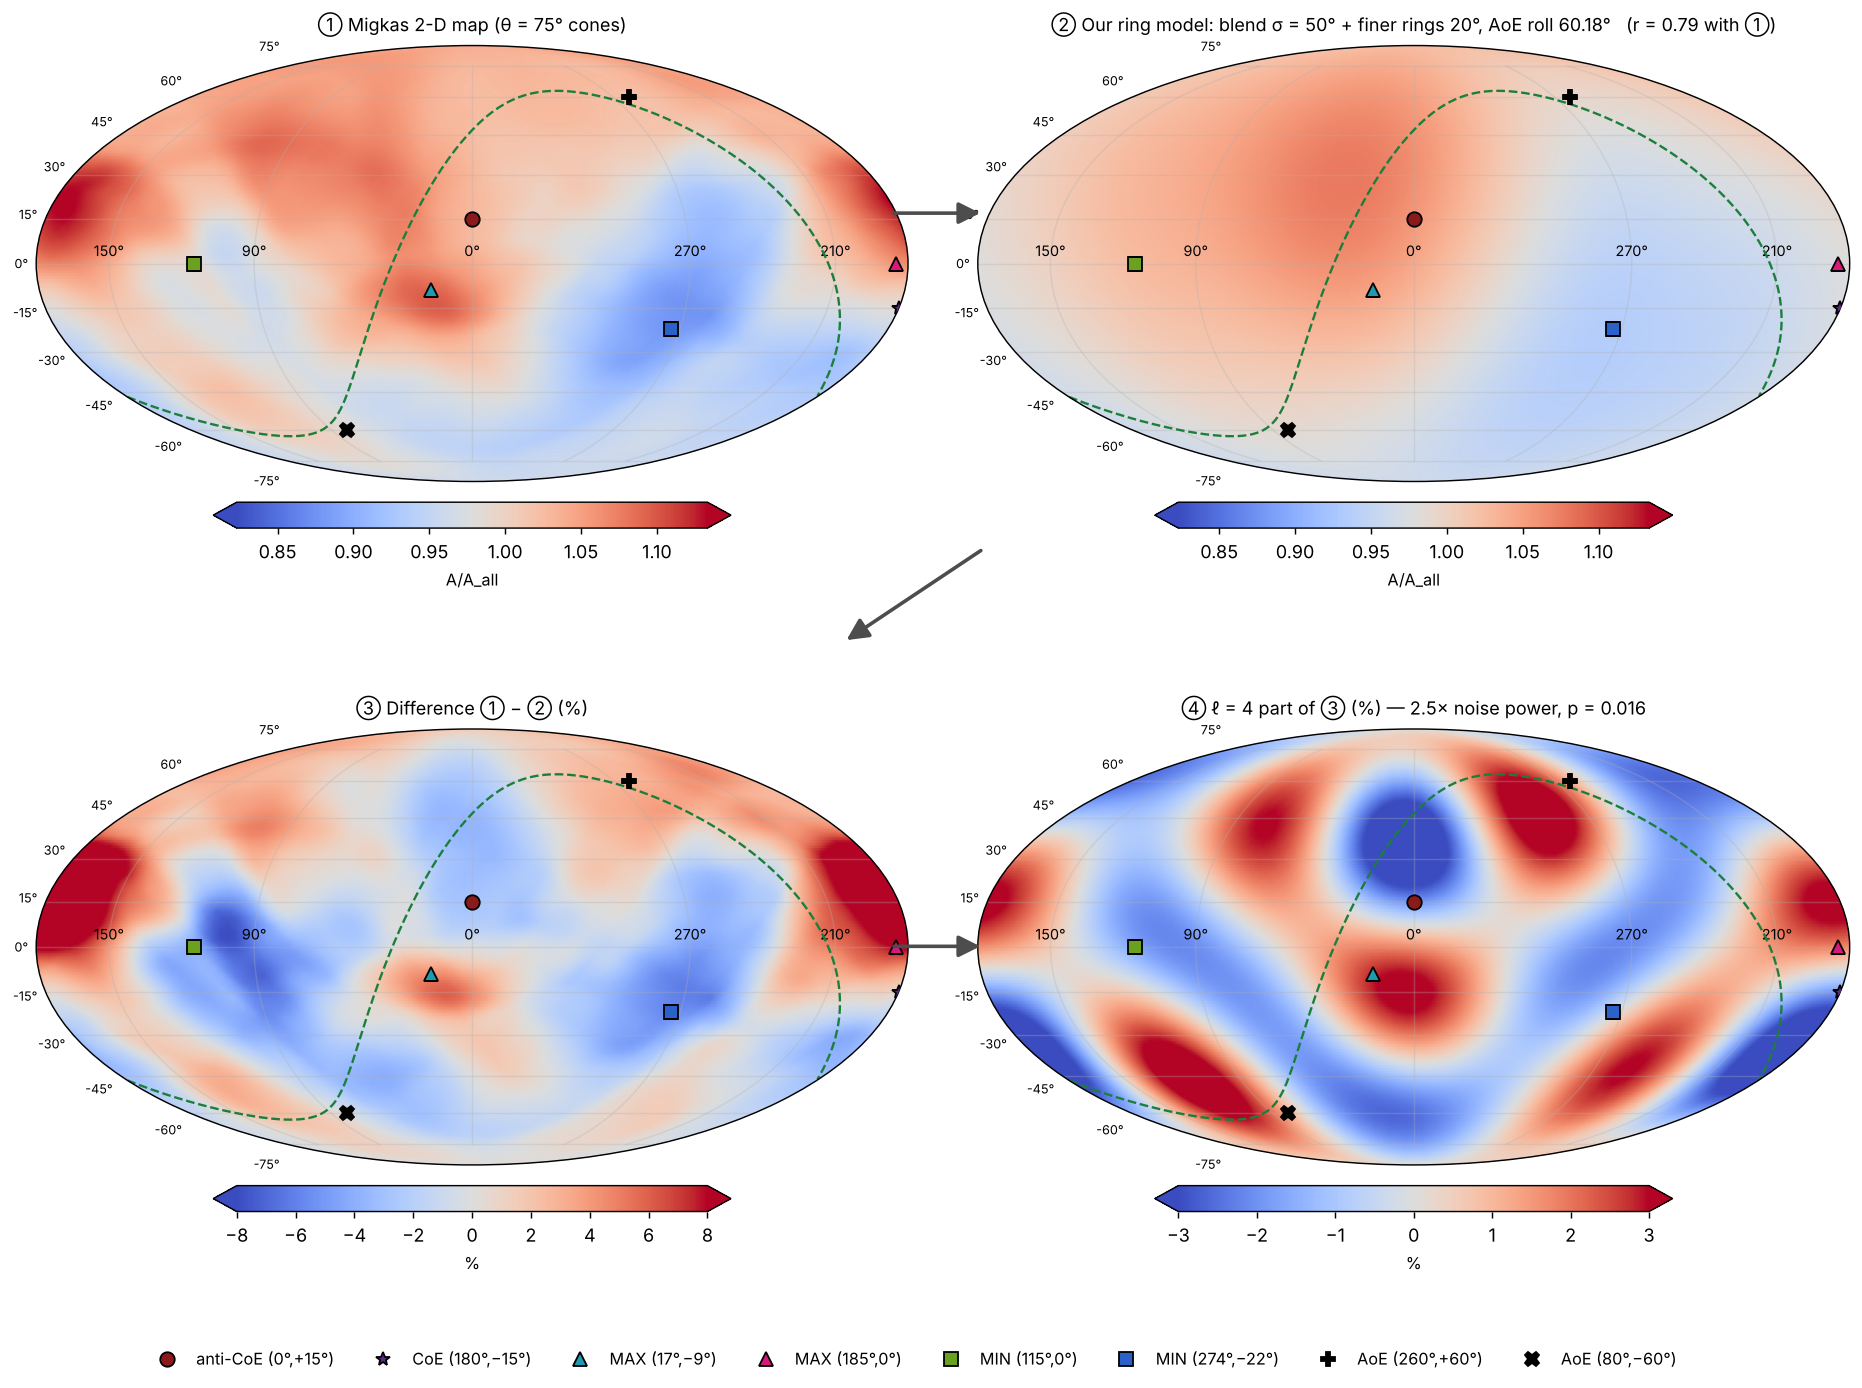
\includegraphics[width=\textwidth,height=0.5\textheight,keepaspectratio]{figs/fig4_chain.png}
\caption{The full chain: (1) Migkas 2-D map; (2) the ring model in the frame; (3) their difference; (4) the $\ell=4$ part of the difference.}\label{fig:chain}
\end{figure}

\begin{figure}[!htb]\centering
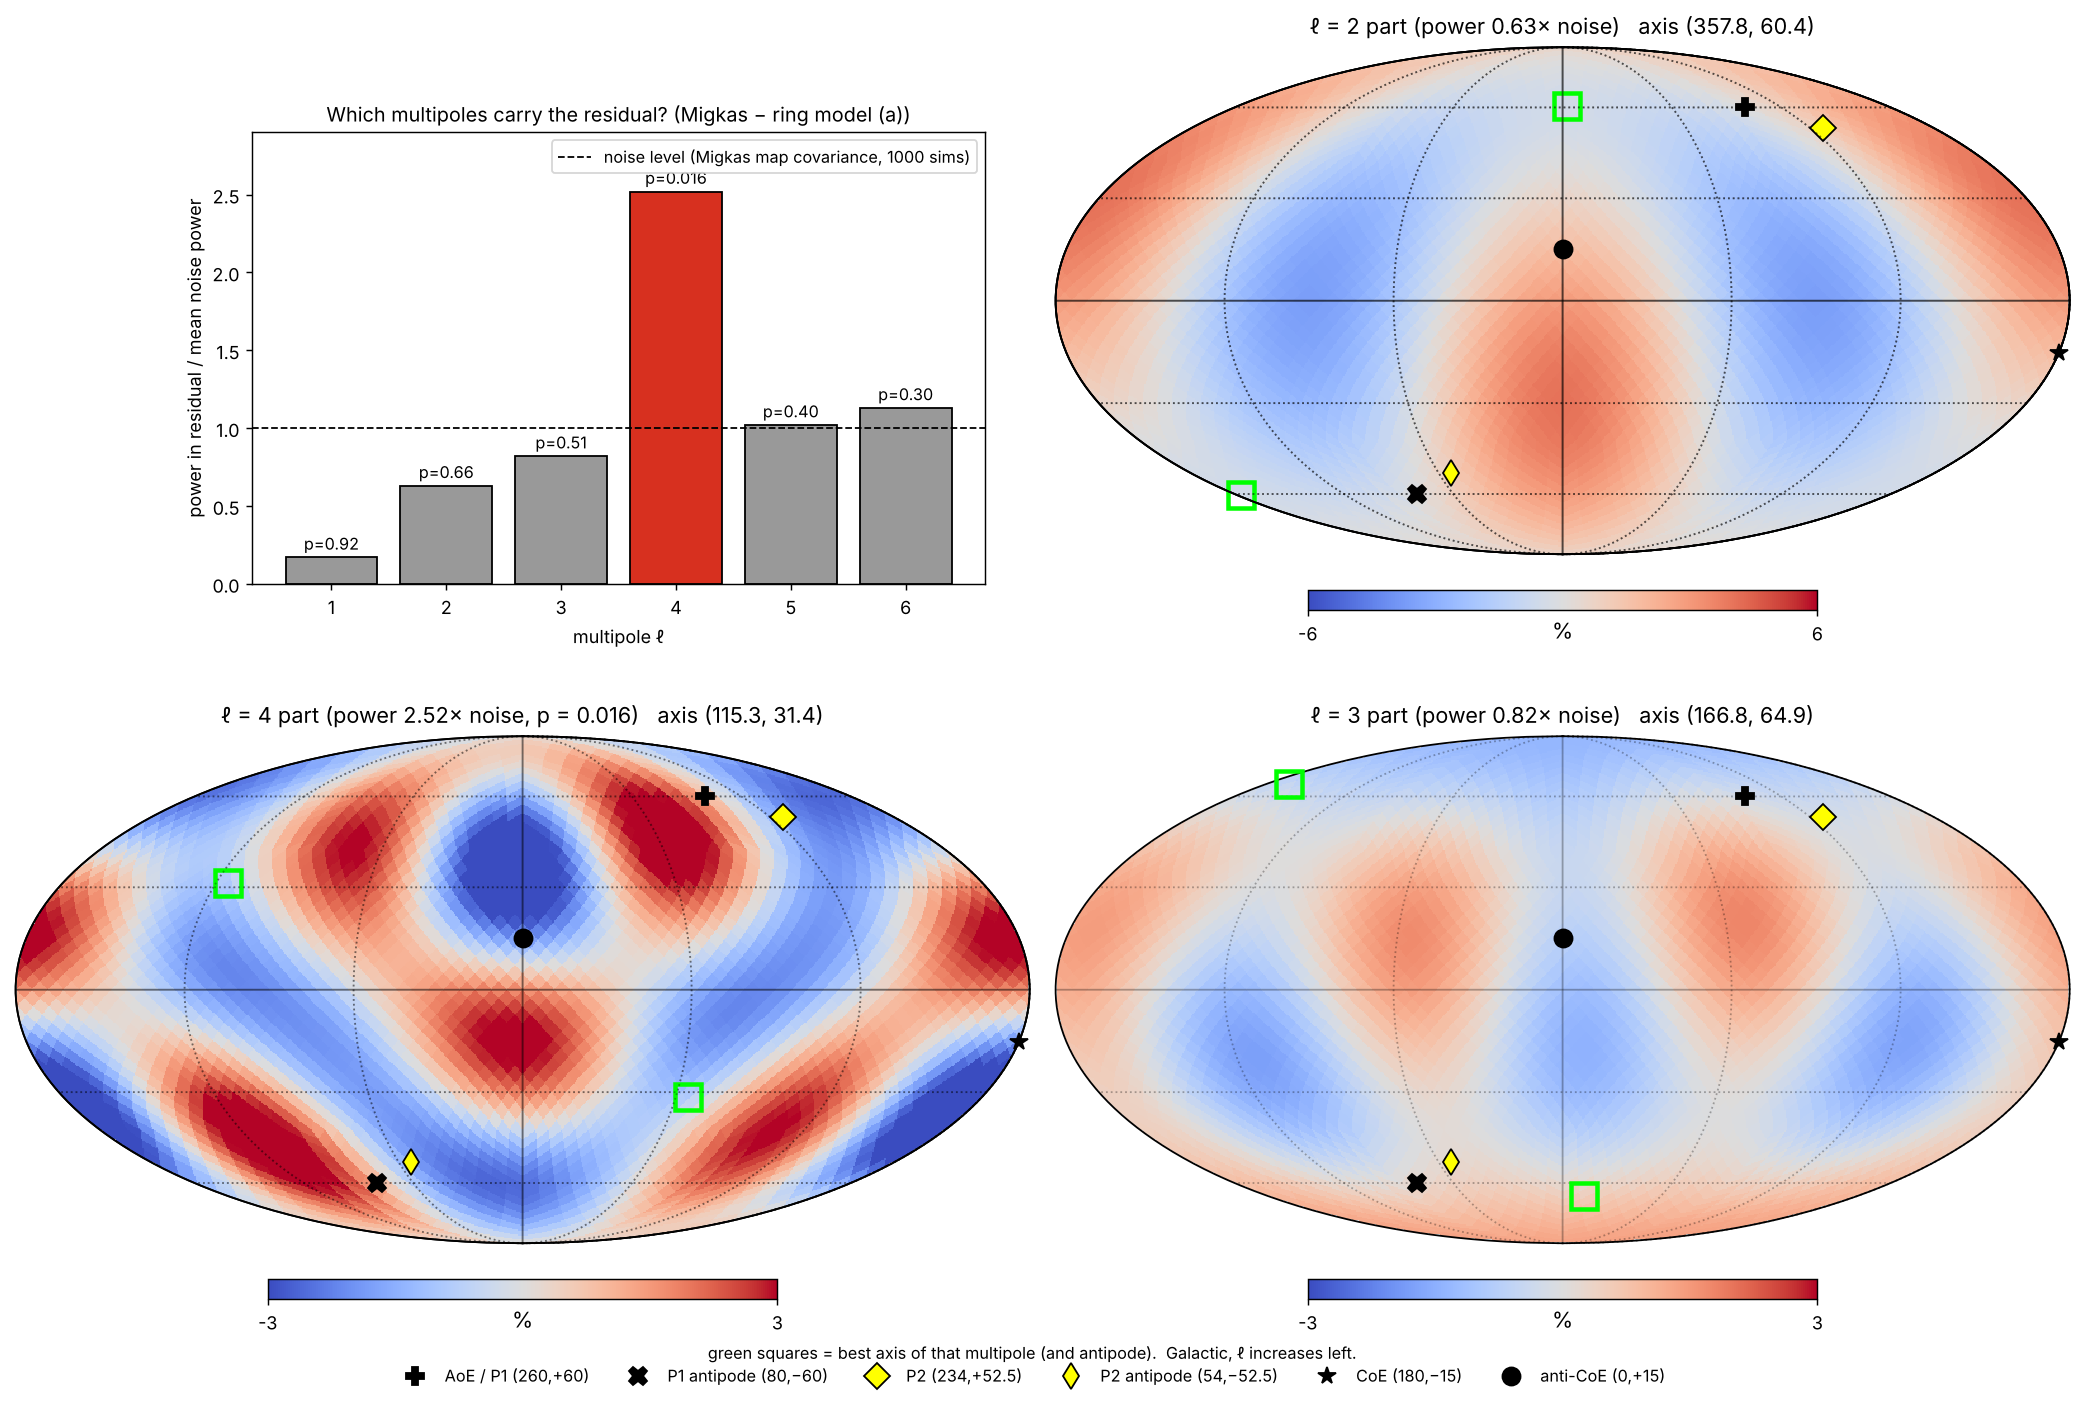
\includegraphics[width=\textwidth,height=0.5\textheight,keepaspectratio]{figs/fig5_multipoles.png}
\caption{Multipole content of the residual. Only $\ell=4$ exceeds the noise level. Green squares: best axis of each multipole and its antipode.}\label{fig:multipoles}
\end{figure}





\section{Evidence, by when it entered the work}\label{sec:tests}
\paragraph{Tier A: predicted before the data.} (Robustness of these numbers to correlated bins: Appendix~\ref{app:robust}.) Observables 1--5 (Table~\ref{tab:origin}) were derived in 2013--16 and hold in every valid setup (Table~\ref{tab:knobs}). Following Migkas et al., the 71 bins of each curve are treated as independent data points with their published errors. Against an isotropic sky (a constant), the CoE model ($D/R=3.56$, seven parameters), improves the fit by $\Delta\chi^2=40.5$ for $A$ (6 extra parameters, $p=3.6\times10^{-7}$, $5.1\sigma$). With $A$ and $B$ computed from one set of inputs (Eqs.~\ref{eq:sheetA}--\ref{eq:sheetB}, Fig.~\ref{fig:AB}), the same $D/R$ gives $\Delta\chi^2=40.2$ for $A$ ($5.1\sigma$) and $30.6$ for $B$; counting all six parameters against $B$, as if none had been fixed by $A$, gives $4.2\sigma$, a lower bound since the inputs are shared. The joint improvement is $\Delta\chi^2=70.9$ for 7 extra parameters ($p=10^{-12}$, $7.1\sigma$), but $A$ and $B$ come from the same clusters, so this joint figure overstates the evidence and is not used as the headline. Against a plain dipole, the CoE model is better for $A$ by $\Delta\chi^2=22.0$ ($3.7\sigma$; see below). The fitted $\chi^2$ per degree of freedom is 0.07 ($A$) and 0.12 ($B$), reflecting the published error bars.

\paragraph{Why compare with a dipole.} Isotropy is the null hypothesis set by the cosmological principle, and the CoE model rejects it at $5\sigma$. A reader who accepts that the cluster sky is anisotropic will then ask whether something more ordinary explains it: our own motion, a bulk flow or an absorption gradient would each produce a dipole, one high and one low, and Migkas et al.\ themselves read their result as near-dipole. The geometry instead predicts two highs and two lows. Figure~\ref{fig:dipole} compares the two on the 71 bins of $A$: the best-fit dipole leaves $\chi^2=26.2$, the CoE geometry $\chi^2=4.2$. The difference, $\Delta\chi^2=22.0$ for four extra parameters ($p=2.0\times10^{-4}$), is $3.7\sigma$. The data prefer a two-maximum, two-minimum pattern over a dipole. That pattern is what the geometry predicted in 2013--14; a generic two-harmonic Fourier series fits about as well (5 parameters, $\chi^2=7.6$; 7 parameters, $\chi^2=3.2$), so the curve alone does not single out the geometry's exact shape over other two-harmonic curves. What it confirms is the predicted form.

\begin{figure}[!htb]\centering
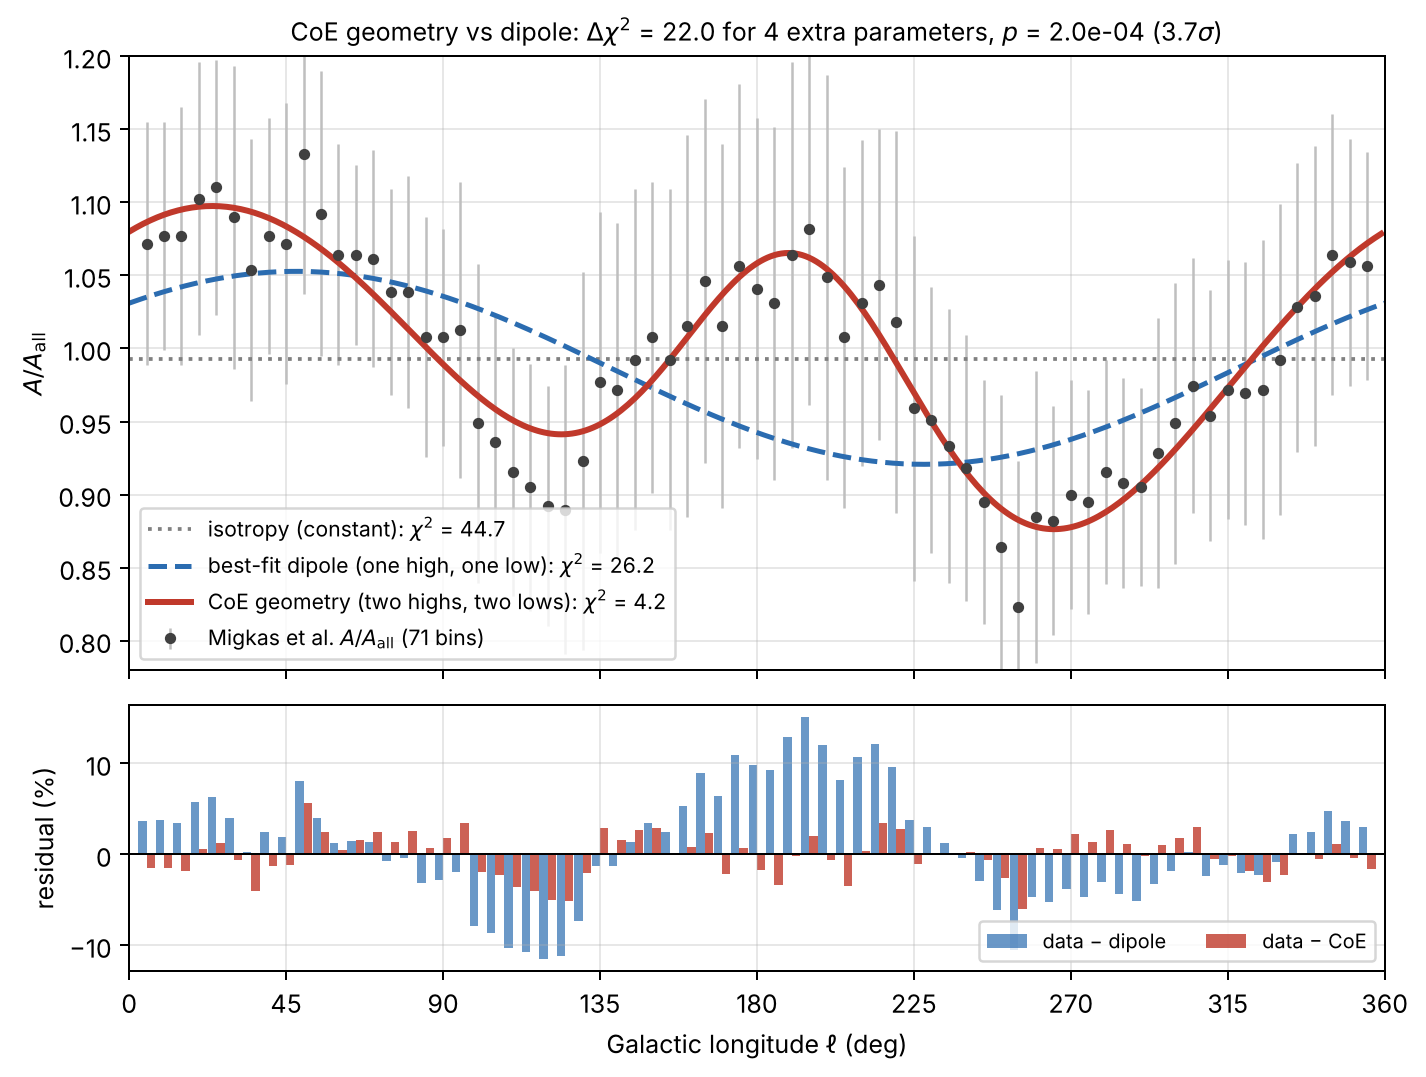
\includegraphics[width=0.82\textwidth]{figs/fig_dipole_cmp.png}
\caption{Migkas $A/A_{\rm all}$ with three models: isotropy ($\chi^2=44.7$), the best-fit dipole ($\chi^2=26.2$) and the CoE geometry ($\chi^2=4.2$). The dipole misses the second maximum near $\ell\approx190\dg$ and the minimum near $120\dg$ (bottom: residuals). The CoE geometry is preferred over the dipole by $\Delta\chi^2=22.0$ for 4 extra parameters, $3.7\sigma$.}\label{fig:dipole}
\end{figure}

\paragraph{Tier B: identified, not built in.} The critical points are a property of the geometry, and the Axis of Evil was compared to them only after they were found. Before the comparison the Migkas fit had fixed $D/R\approx3$--4.5 and a roll of $45$--$80.8\dg$. With the CoE direction fixed, a random headless axis falls inside that patch (either roll branch) with probability 1.1\% (2--6: 3.2\%; 2--8: 3.6\%; $2\times10^6$ random axes). The Axis of Evil lies inside it, at $\theta_0=81.94\dg$ and roll $60.18\dg$. The roll window used no CMB information: its $80.8\dg$ end was fitted to the four Migkas maximum and minimum positions, and no roll was ever adjusted to a CMB feature. The model's second direction and plane also existed before the author learned that the CMB requires a preferred plane with broken internal symmetry \cite{RS07}; the frame supplied that structure before the requirement was known.

\paragraph{Tier C: tested after the frame was fixed.} Three statistics, fixed before the run: T1, feature signs (11 of 12); T2, the $\ell=4$ belt axis $14.8\dg$ from the plane-of-evil normal; T3, the map's best roll $50\dg$ against $60.18\dg$. Null~A rotates the whole frame; null~B keeps the Axis of Evil fixed and places the CoE at random, measuring what the CoE adds (Table~\ref{tab:sig}, Fig.~\ref{fig:nulls}). Tier B and tier C cannot be combined, because tier C uses the Axis of Evil as an input. T3 counts both roll branches ($60.18\dg$ and $240.18\dg$), as tier B does. The 12 features and their scores are listed in Table~\ref{tab:features} and shown in Fig.~\ref{fig:spots}; Fig.~\ref{fig:dipoles} shows the published dipoles in the frame.

\begin{table}[!htb]\centering\small
\caption{Tier C significance (20\,000 draws per null). Null B is the fair measure of the CoE claim.}\label{tab:sig}
\setlength{\tabcolsep}{4pt}
\begin{tabular}{lcc}\toprule
Test & Null A: whole frame random & Null B: CoE random, AoE fixed\\\midrule
T1 feature signs (11/12) & $p=0.015$ & $p=0.023$\\
T2 $\ell=4$ axis to plane normal ($14.8\dg$) & $p=0.032$ & $p=0.150$\\
T1 + T2 joint & $p=0.0034$ ($2.9\sigma$) & $p=0.020$ ($2.3\sigma$)\\
T3 roll within $10.2\dg$ (either branch) & $p=0.113$ & $p=0.113$\\
All three & $p=0.0034$ ($2.9\sigma$) & $p=0.016$ ($2.4\sigma$)\\\bottomrule
\end{tabular}
\end{table}

\begin{figure}[!htb]\centering
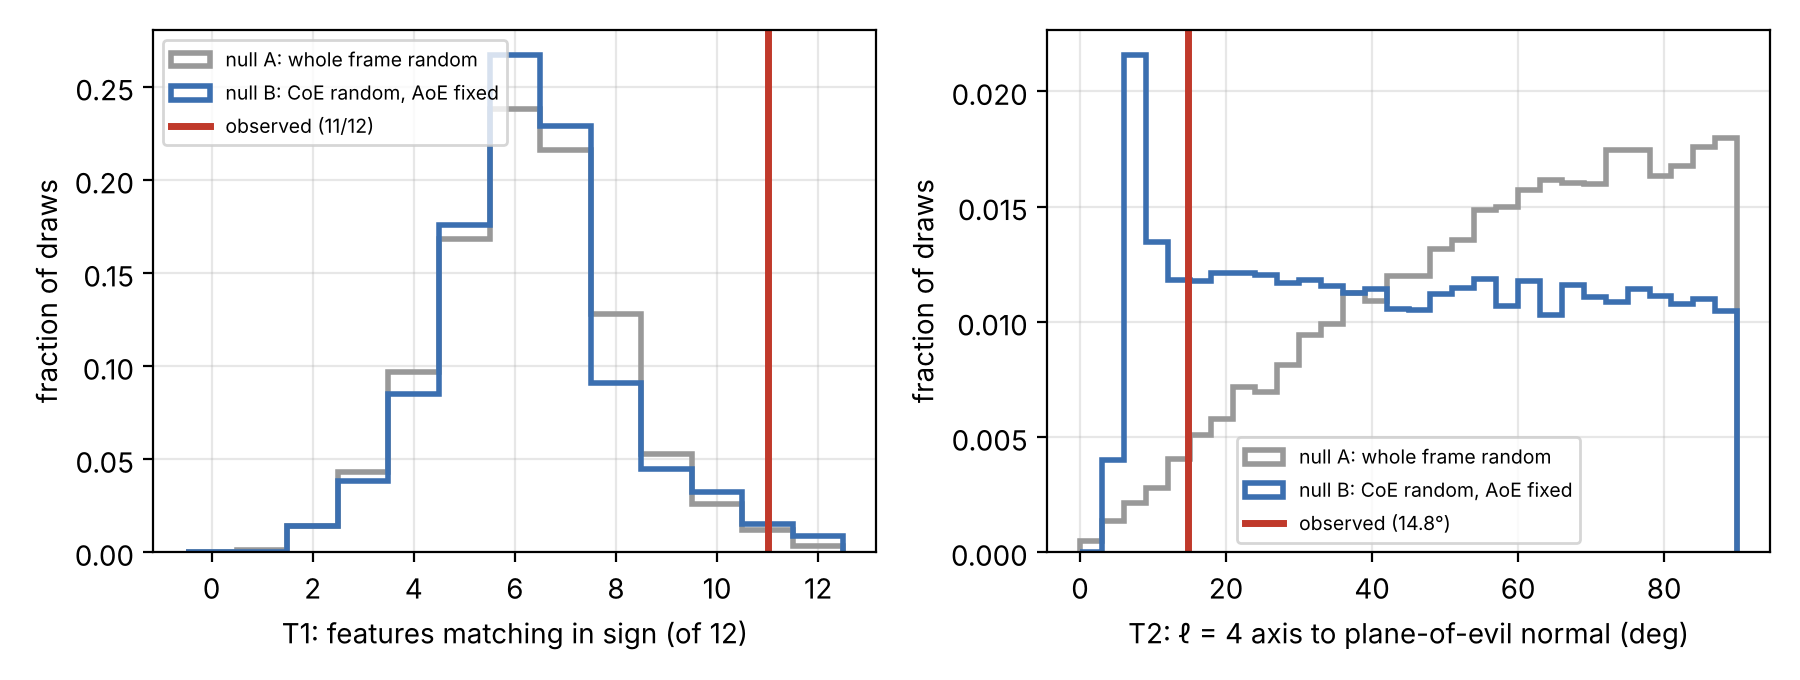
\includegraphics[width=0.88\textwidth]{figs/fig6_nulls.png}
\caption{Null distributions of T1 and T2 for both nulls, with the observed values.}\label{fig:nulls}
\end{figure}

\begin{figure}[!htb]\centering
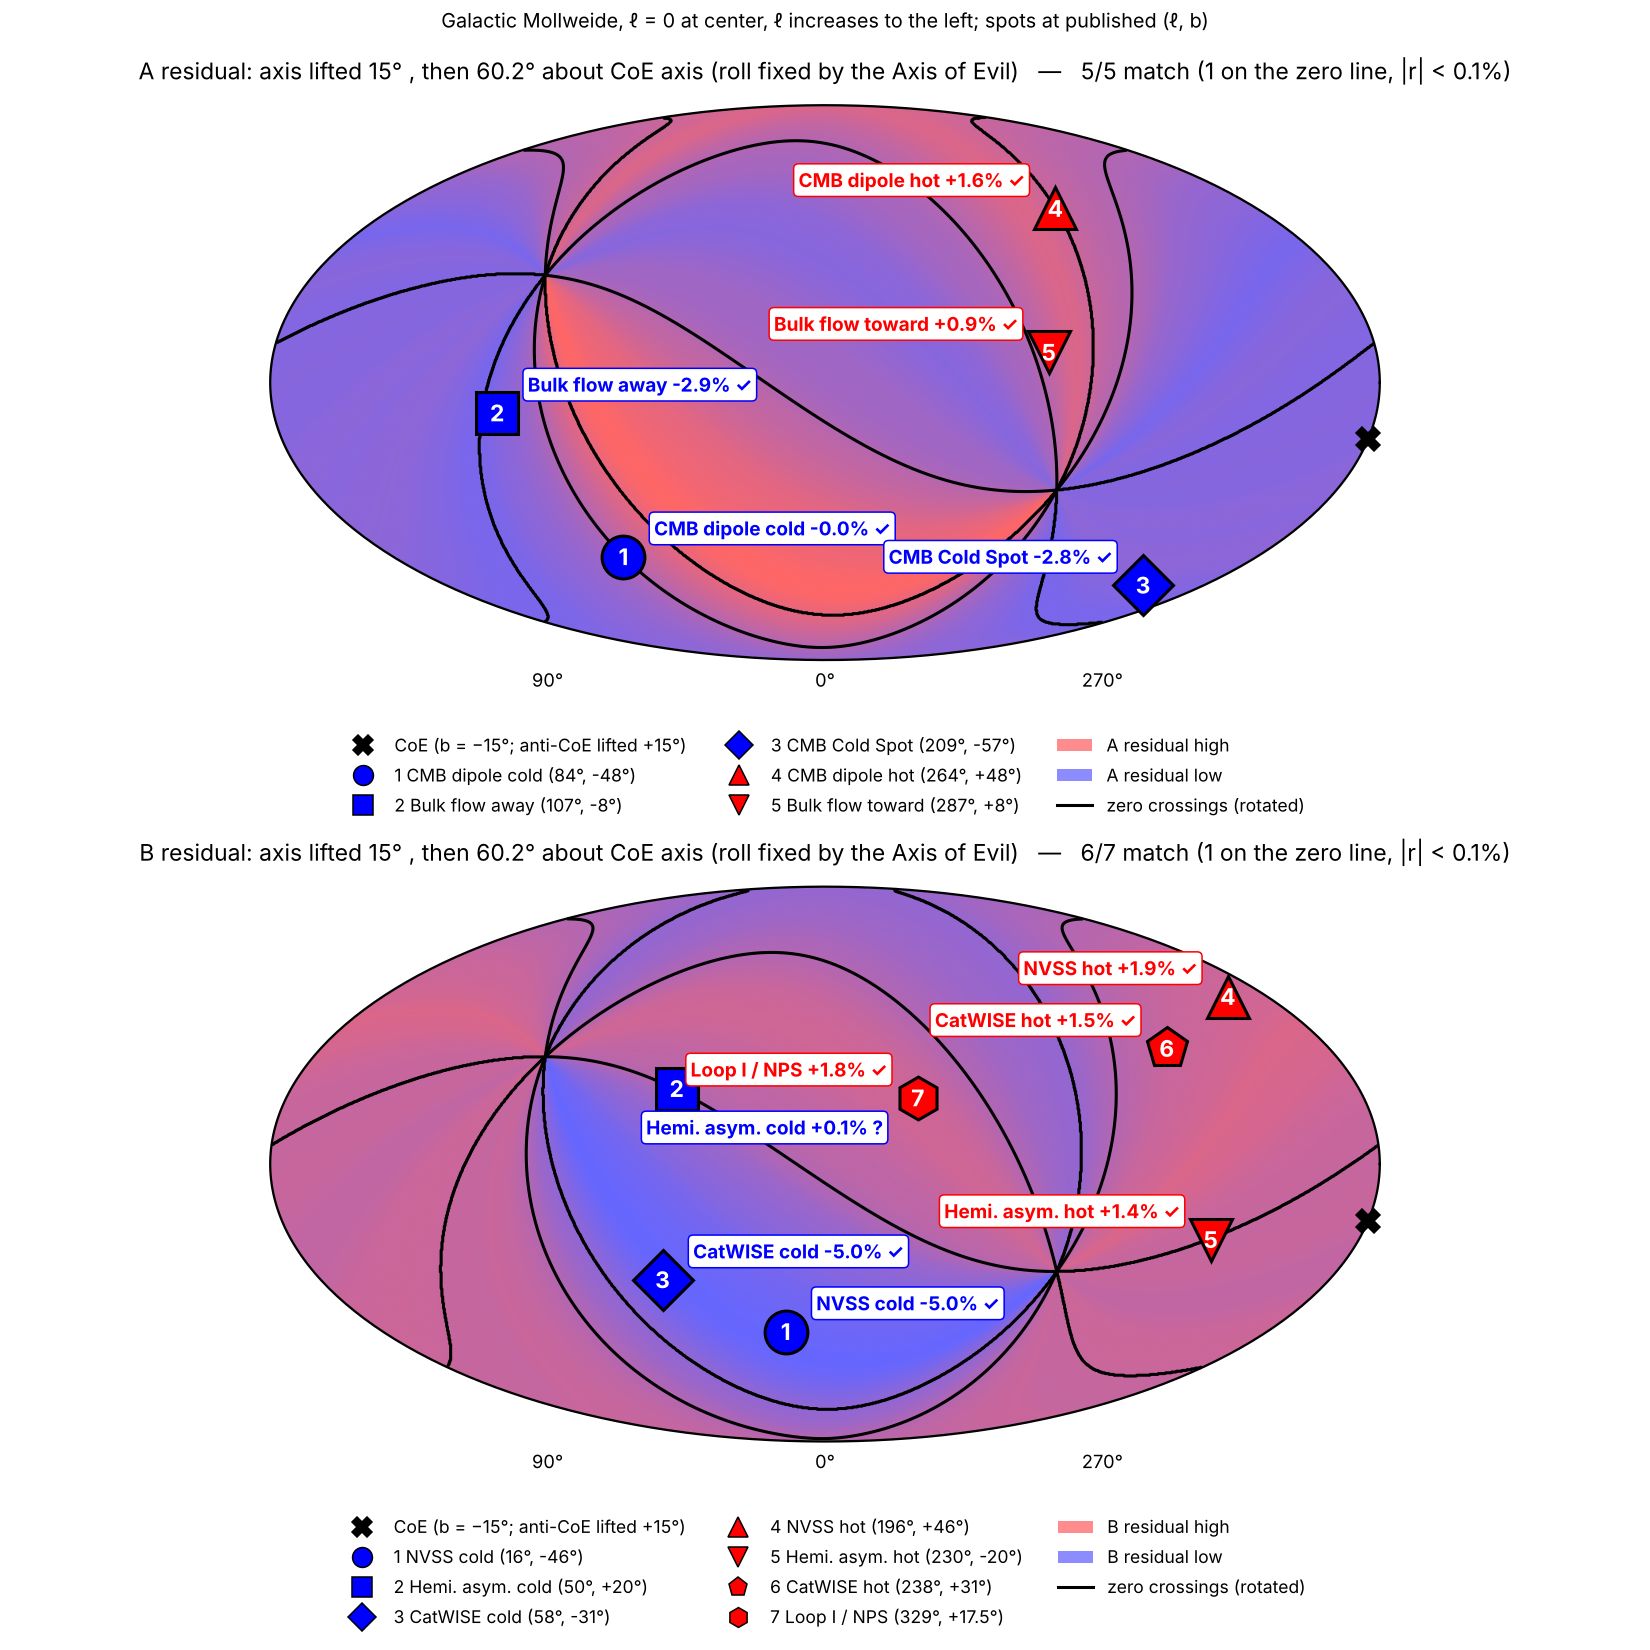
\includegraphics[width=0.86\textwidth]{figs/fig_spots.png}
\caption{Residual maps of $A$ (top) and $B$ (bottom) in the Axis-of-Evil frame, red above and blue below the model, with zero crossings. Each anomaly feature sits on the side matching its sign in 11 of 12 cases (T1).}\label{fig:spots}
\end{figure}
\begin{table}[!htb]\centering\small
\caption{The 12 features in the residual maps (Fig.~\ref{fig:spots}): published direction, expected sign, residual at the feature's frame position, and the zone it falls in: 10 clear matches, 1 marginal match on the zero line, 1 miss (11 of 12 by sign).}\label{tab:features}
\setlength{\tabcolsep}{4pt}
\begin{tabular}{llllrll}\toprule
Map & Feature & $(l,b)$ & Expected & Resid.\ (\%) & Zone & Match\\\midrule
A & CMB dipole, cold end & $(84\dg, -48\dg)$ & cold & -0.01 & low & marginal$^{a}$\\
A & Bulk flow, away & $(107\dg, -8\dg)$ & cold & -2.86 & low & yes\\
A & CMB Cold Spot & $(209\dg, -57\dg)$ & cold & -2.78 & low & yes\\
A & CMB dipole, hot end & $(264\dg, +48\dg)$ & hot & +1.56 & high & yes\\
A & Bulk flow, toward & $(287\dg, +8\dg)$ & hot & +0.93 & high & yes\\
B & NVSS dipole, cold end & $(16\dg, -46\dg)$ & cold & -5.05 & low & yes\\
B & Hemisph.\ asym., cold & $(50\dg, +20\dg)$ & cold & +0.06 & zero$^{a}$ & no\\
B & CatWISE dipole, cold end & $(58\dg, -31\dg)$ & cold & -5.02 & low & yes\\
B & NVSS dipole, hot end & $(196\dg, +46\dg)$ & hot & +1.87 & high & yes\\
B & Hemisph.\ asym., hot & $(230\dg, -20\dg)$ & hot & +1.36 & high & yes\\
B & CatWISE dipole, hot end & $(238\dg, +31\dg)^{b}$ & hot & +1.48 & high & yes\\
B & Loop I / NPS & $(329\dg, +17.5\dg)$ & hot & +1.84 & high & yes\\
\bottomrule
\multicolumn{7}{l}{\footnotesize $^{a}$ Within 0.1\% of zero; the test scores by sign, as fixed before it was run.}\\
\multicolumn{7}{l}{\footnotesize $^{b}$ Catalog value used in the test; Secrest et al.\ give $(238.2\dg,+28.8\dg)$, used in Fig.~\ref{fig:dipoles}. The sign is unchanged.}\\
\end{tabular}
\end{table}


\begin{figure}[!htb]\centering
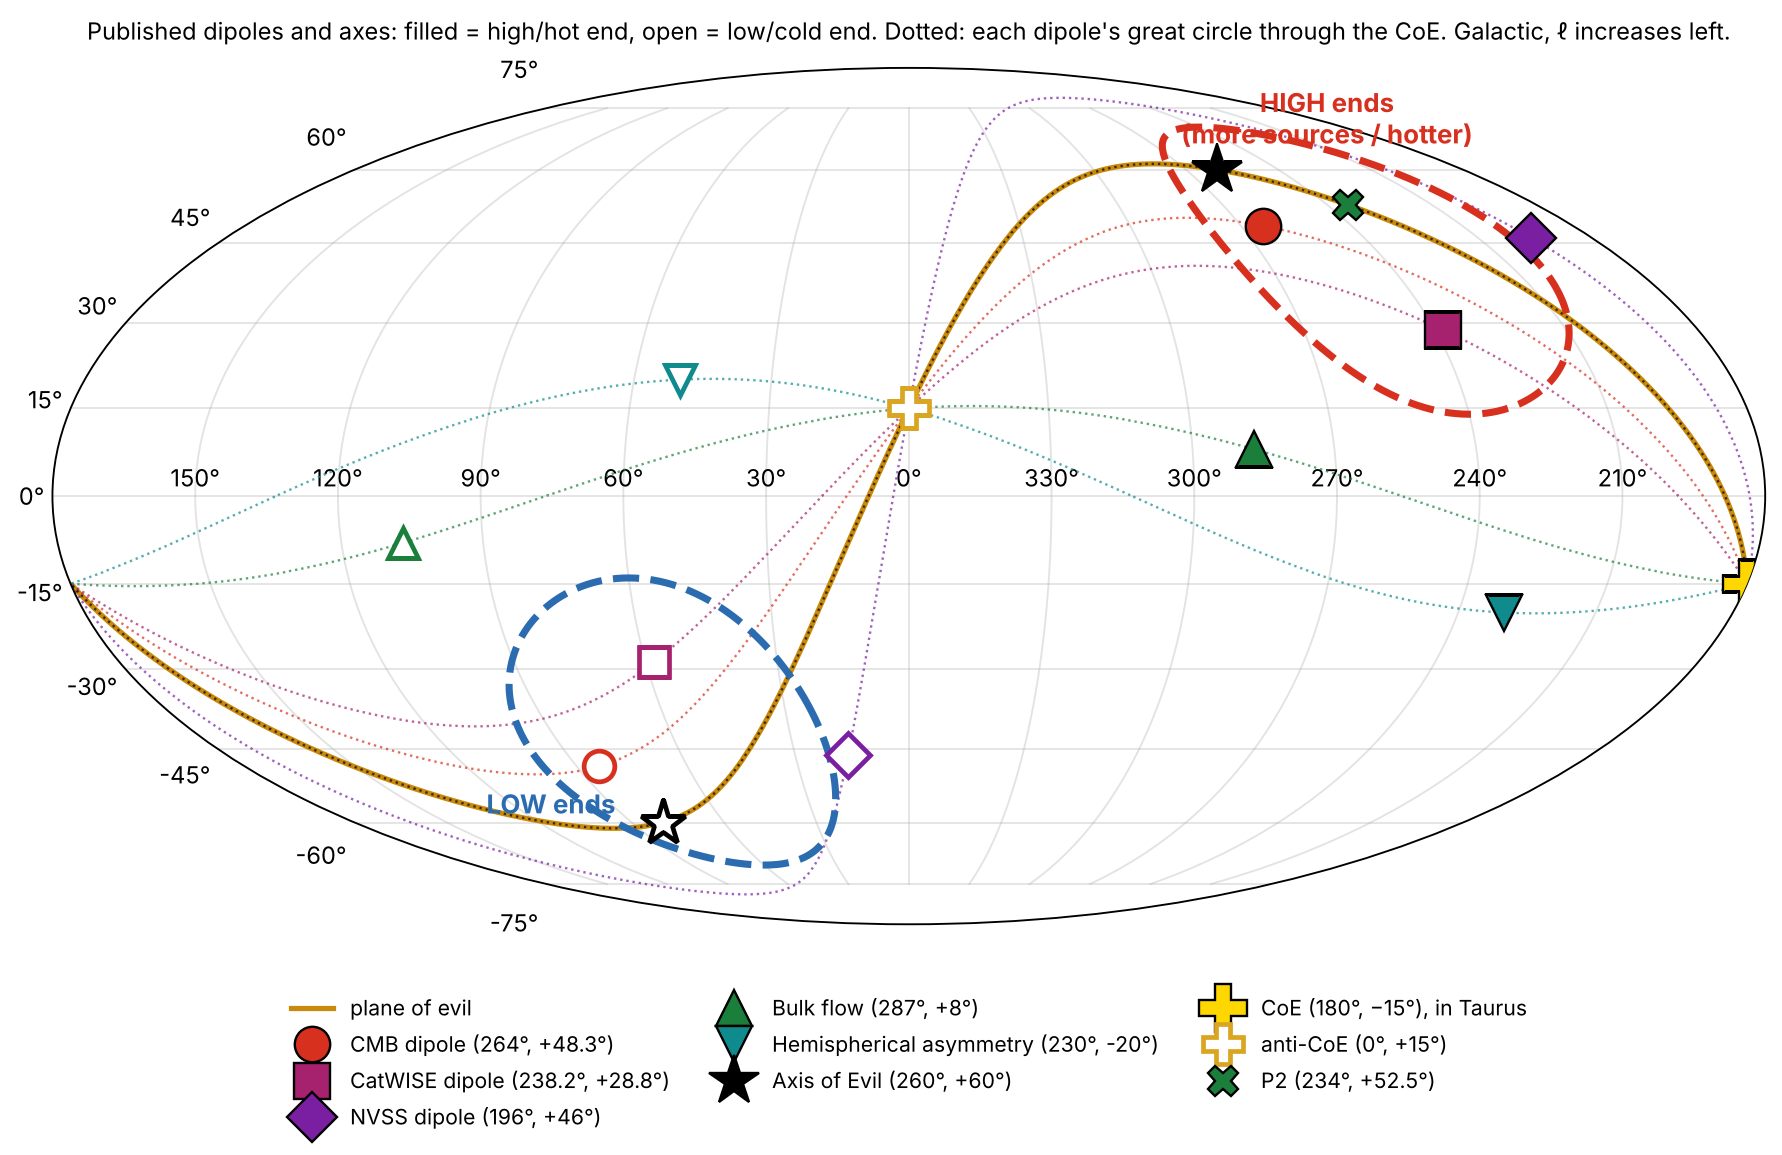
\includegraphics[width=0.9\textwidth]{figs/fig_dipoles.png}
\caption{Published dipoles and axes: filled markers are the high (hot, more sources) ends, open markers the low ends. Dotted lines join each dipole to the CoE along a great circle. The high ends cluster around the Axis of Evil and P2 on the plane of evil (red circle); the low ends cluster around the opposite pole (blue).}\label{fig:dipoles}
\end{figure}

\paragraph{Other axes in the frame} (observations, not counted). The CMB dipole $(264\dg,+48\dg)$ and the Copi et al.\ quadrupole normal $(231.7\dg,+63\dg)$ lie $12\dg$ and $9\dg$ from the plane of evil, but only because they lie near the Axis of Evil. The hemispherical-asymmetry axis $(230\dg,-20\dg)$ lies $48\dg$ from the CoE axis, $12\dg$ from the multipole plane of the geometry (normal to P1--P2) and $6\dg$ from the plane normal to the published headless axis.

\section{What breaks the symmetry}\label{sec:sym}
A radially symmetric CoE cannot produce the observed multipoles. Symmetric surroundings give only patterns symmetric about the CoE axis; the quadrupole and octopole are instead planar about the Axis of Evil, with their in-plane symmetry broken \cite{RS07}. In the geometry the P1--P2 axis is exactly perpendicular to the CoE, so the CoE lies in the multipole plane. The published headless axis lies $82\dg$ rather than $90\dg$ from the CoE; the $8\dg$ difference is what a headless fit to a pattern with non-antipodal ends would give, and it is within the $10$--$15\dg$ spread of published axes. The region around the CoE must therefore carry a second direction of its own: a flattened matter distribution, rotation of the expanding region, or shear.

\paragraph{The Bianchi VII$_h$ precedent.} Bianchi VII$_h$ universes are uniform but anisotropic: they expand at different rates along different axes (shear) and rotate (vorticity), which focuses CMB light into a spiral pattern. Jaffe et al.\ \cite{Jaffe05} found a Bianchi VII$_h$ template in the WMAP sky at about $3\sigma$, with axis near $(222\dg,-62\dg)$; subtracting it reduced the power asymmetry and could also address the low quadrupole and the Cold Spot, and it persisted in the three-year data \cite{Jaffe06}. It required an open, low-density universe incompatible with the acoustic peaks, and Planck \cite{Planck13XXVI} found no evidence for a physically consistent Bianchi VII$_h$ cosmology. The lesson is that the mechanism, not only the pattern, must fit the power spectrum and the expansion history. In our frame the Bianchi axis lies $55\dg$ from both the Axis of Evil and the CoE axis.

\paragraph{The supernova test.} A pre-registered test of the frame against 490 Pantheon+ supernovae at $0.023<z<0.15$ (full covariance) found the dipole part of the predicted Hubble-rate pattern at the predicted direction and size (amplitude $1.05\pm0.46$ against 1), but not the two-maximum, two-minimum part (amplitude $0.04\pm0.05$ against 1). At these distances the supernovae therefore do not show the even pattern seen in the clusters. Either the Migkas pattern is not mainly an expansion-rate anisotropy at $z<0.15$ (it may reflect cluster-specific effects such as absorption or scaling-relation systematics), or it arises at larger distances than the supernovae sample. This is a failed prediction for the expansion reading and is reported as such.

\section{Where to look}\label{sec:sky}
The center of expansion lies behind Orion (Fig.~\ref{fig:sky}). The direction that best fits the Migkas data, $(l,b)=(198\dg,-4\dg)$, or RA $6^{\rm h}09^{\rm m}$, Dec $+11\dg$, sits about $5\dg$ from Betelgeuse, Orion's red shoulder star, toward Gemini. It is in the winter evening sky of the northern hemisphere, and the CoE itself lies far beyond any visible star. For reference, the direction $(180\dg,-15\dg)$ used to set up the frame lies about $20\dg$ away, in Taurus beside Aldebaran. Opposite, the anti-CoE lies in Serpens, in the summer sky. The Axis of Evil points toward Leo (about $11\dg$ from Denebola) and Aquarius; P2 lies about $6\dg$ from Regulus; the plane of evil's pole points toward Draco and Dorado.

\begin{figure}[!htb]\centering
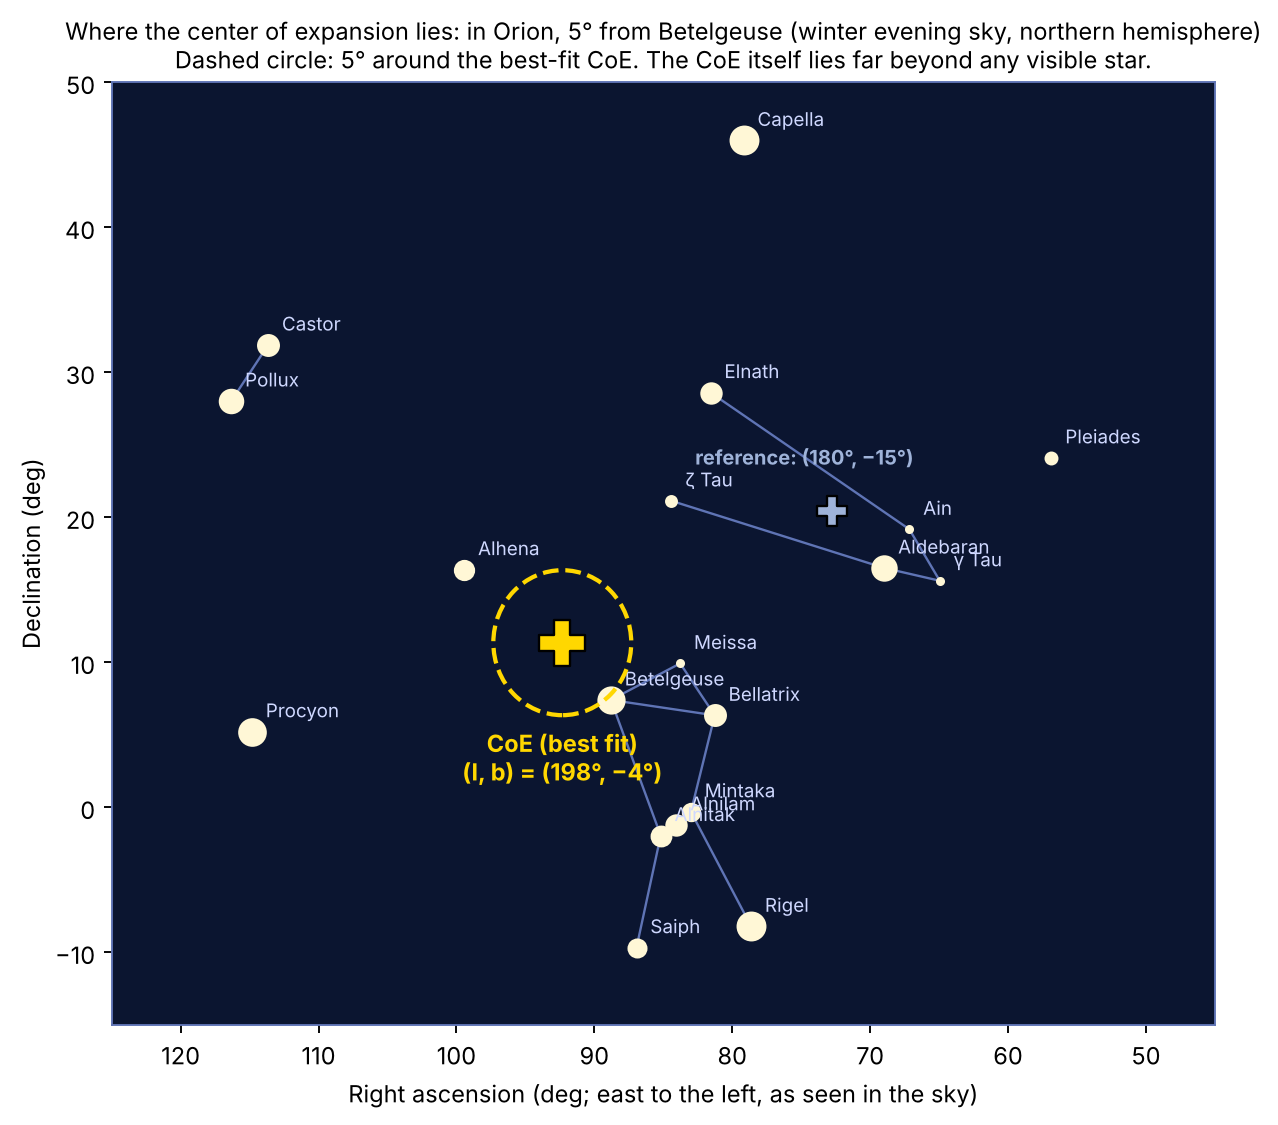
\includegraphics[width=0.7\textwidth]{figs/fig_sky.png}
\caption{The best-fit CoE direction among the stars of Orion and Taurus, $5\dg$ from Betelgeuse (dashed circle: $5\dg$). The reference direction $(180\dg,-15\dg)$ is marked near Aldebaran.}\label{fig:sky}
\end{figure}

\section{The CMB: one test made, the amplitudes still open}\label{sec:cmb}
\paragraph{The multipole plane in Planck.} Raki\'c \& Schwarz \cite{RS07} showed that the low-$\ell$ alignments require a preferred plane, with the Axis of Evil as its normal and no rotational symmetry within the plane; they do not say which direction in the plane is preferred. The geometry supplies such a plane: normal to the P1--P2 axis, perpendicular to the plane of evil, and containing the CoE (Section~\ref{sec:geom}). It predicts that a measured multipole axis lies at the P1--P2 axis, $90\dg$ from the CoE, rather than at the published headless axis, $82\dg$ from it. We measured the quadrupole--octopole axis in the Planck PR3 SMICA map \cite{Planck18IV} with the Land \& Magueijo statistic \cite{LM05} (Appendix~\ref{app:smica}). On the full sky the combined $\ell=2,3$ axis is $(238.7\dg,+60.5\dg)$: $5.1\dg$ from the P1--P2 axis and $10.5\dg$ from the published axis $(260\dg,+60\dg)$. The CoE lies $1.3\dg$ from the measured plane ($0.1\dg$ for the octopole alone). With the Galactic plane masked ($|b|>10\dg$, $|b|>20\dg$) the axis stays $2.2$--$5.3\dg$ from the P1--P2 axis and the CoE $0.2$--$4.9\dg$ from the plane. A random direction lies within $5\dg$ of a given plane with probability $\approx9\%$, within $1.3\dg$ with $\approx2\%$. This prediction was in the draft (Section~\ref{sec:concl}) before the map was examined.

The measured multipoles have the structure the frame requires. Both are almost purely sectoral about the measured axis (99\% of the $\ell=2$ power, 93\% of $\ell=3$): planar, with the rotational symmetry within the plane broken, as Raki\'c \& Schwarz found \cite{RS07}. The geometry fixes the plane and its normal; in its present form it does not fix the azimuth of the lobes within the plane. For reference, the CoE lies $28\dg$ from the nearest quadrupole extremum and $18.6\dg$ from the nearest octopole extremum, values a fuller model of the CoE region (flattening or rotation) would have to reproduce. The 2-D Migkas best-fit CoE $(198\dg,-4\dg)$ lies $16$--$22\dg$ from the measured plane; the frame CoE $(180\dg,-15\dg)$ is the one the CMB favors.

\paragraph{The amplitudes.} The CoE geometry alone gives a strongly anisotropic CMB. A web of structure along the line of sight can cancel much of that anisotropy multipole by multipole, posed as an inverse problem. Early versions bring the predicted sky closer to what is observed; no quantitative CMB result is claimed. We expect diffusion-like structures to have formed in the plasma before recombination; their fingerprint should be recoverable from the residual left after the systematic cancellation. This is the largest open problem in the program.

\section{Relation to earlier work}
The ingredients are established: the anomalies \cite{Schwarz04,Copi07,LM05,Secrest21,Migkas20}, the requirement for a preferred plane \cite{RS07}, anisotropic cosmologies \cite{Jaffe05,Planck13XXVI}, off-center observers in LTB universes \cite{Alnes06}, and superhorizon perturbations as a source of large-scale asymmetry \cite{Erickcek08}. Closest to the starting question of this work, Smoller and Temple constructed exact solutions of the Einstein equations in which the Big Bang is a localized explosion behind an outgoing shock wave, inside a white hole of finite mass \cite{ST03}, and a one-parameter family of expanding-wave solutions containing the radiation-era Friedmann model in which every other member has a center of expansion and produces an apparent acceleration without a cosmological constant \cite{ST09}; evolved to the present, these give an acceleration that differs from dark energy at third order in redshift \cite{STV17}. Those solutions place the observer at the center; Smoller and Temple note that an observer away from it would see large angular variations in the expansion rate \cite{ST09}. The geometry here computes that off-center signature, $A(\theta)$, for a center beyond the observable sphere, and compares it with the cluster data. The isotropy limit they cite for a center inside the visible universe (an observer within about 15\,Mpc of it) does not apply directly when the center lies outside, where the effect is a large-scale gradient; whether that gradient is consistent with the CMB dipole and quadrupole is the amplitude question of Section~\ref{sec:cmb}. An unreviewed preprint \cite{Bao23} places a center inside the observable universe at $(286\dg,-43\dg)$, about $90\dg$ from our CoE and about $15\dg$ from our plane-of-evil normal. To our knowledge the construction here has not been published; a full literature search is needed before submission.

\section{Limitations}
\begin{itemize}\setlength\itemsep{1pt}
\item \textbf{Inputs.} The frame uses the CoE direction $(180\dg,-15\dg)$ from the original sky-orientation work (the latitude chosen to place the anti-CoE at $b=+15\dg$). Rebuilding the frame on the 2-D best fit $(198\dg,-4\dg)$ gives $D/R=2.88$, improves T2 ($6.7\dg$, $p=0.007$) but lowers T1 to 7/12 ($p\approx0.43$); the null-B joint becomes $p=0.075$. A direction fitted to the cluster map and the feature catalog together is future work. Published Axis-of-Evil axes differ by $10$--$15\dg$.
\item \textbf{Shared data.} Tier C tests all use the 313 Migkas clusters and are not fully independent.
\item \textbf{Map smoothing.} The $75\dg$ cones spread power between multipoles; part of the $\ell=4$ excess may come from that.
\item \textbf{Records.} Tier A depends on dated records of the prior predictions.
\item \textbf{WMAP and Planck axes.} The published axis $(260\dg,+60\dg)$ comes from WMAP-era data; part of its $8$--$13\dg$ offset from the SMICA axis may reflect data and method rather than the geometry. A comparison with Planck's own published low-$\ell$ axes is still to be made. The non-antipodal ends cannot be tested with pure $\ell=2,3$ harmonics, which are symmetric under inversion; that needs localized statistics.
\item \textbf{Supernovae.} The even (two-maximum) part of the pattern is absent in Pantheon+ at $z<0.15$ (Section~\ref{sec:sym}).
\end{itemize}

\section{Conclusions and falsifiable predictions}\label{sec:concl}
The cluster anisotropy rejects isotropy at $5\sigma$ under the CoE geometry (at least $2.6\sigma$ with bin correlations included), adding to the evidence that the cosmological principle does not hold strictly at the largest scales. A geometry explored for another purpose has robust features, a two-pole maximum and a minimum ring on its critical circle, that appear in independent cluster data, and critical points that coincide with the Axis of Evil. The Axis of Evil falls inside the patch the cluster data had fixed (about 1\%), and the resulting frame passes further tests at $2.4\sigma$ for the CoE alone; the cluster curves themselves favor the CoE pattern over isotropy at $5\sigma$ and its two-maximum form over a dipole at $3.7\sigma$ (Section~\ref{sec:tests}). Predictions to be fixed before the data are examined:
\begin{enumerate}\setlength\itemsep{1pt}
\item \textbf{Planck SMICA:} the low-$\ell$ multipoles are planar, with broken symmetry within the plane, about an axis at the P1--P2 axis. \emph{Tested: consistent} (93--99\% sectoral about an axis $2$--$5\dg$ from P1--P2; Section~\ref{sec:cmb}).
\item \textbf{eROSITA clusters:} a minimum ring on the critical circle, and the $\ell=4$ belt near the plane of evil, in an independent sample.
\item \textbf{Non-antipodal Axis of Evil:} measured separately in a Planck map, the two end-regions of the low-$\ell$ alignment are $2\theta_0\approx164\dg$ apart, not $180\dg$, both displaced about $8\dg$ toward the CoE. Their separation measures $D/R$ from the CMB alone; a separation consistent with $180\dg$ would rule out the P1--P2 reading.
\item \textbf{CoE in the multipole plane:} with the P1--P2 axis as the true axis, the CoE lies in the quadrupole/octopole plane to within the measurement errors. \emph{Tested: passed} in Planck SMICA, CoE $0.2$--$4.9\dg$ from the measured plane (Section~\ref{sec:cmb}).
\item \textbf{Flattened-CoE model:} one setting reproduces the multipole orientation, the $\ell=4$ amplitude and the absence of the even pattern in supernovae together.
\end{enumerate}

\section*{Acknowledgments}
I thank Dr.\ Rindler for the time he gave me after his evening graduate classes. The hours ran late, but we had fun working through this geometry together.

\appendix
\section{Prior observables and their dates}\label{app:origin}
\begin{table}[H]\centering\small
\caption{Observables of the geometry, when they were derived, and their later observation. Dates are the author's recollection, to be confirmed against dated records.}\label{tab:origin}
\begin{tabularx}{\textwidth}{>{\raggedright\arraybackslash}p{4.3cm}>{\raggedright\arraybackslash}p{2.0cm}>{\raggedright\arraybackslash}X>{\raggedright\arraybackslash}p{3.4cm}}\toprule
Observable & Derived & Form at the time & Later observation\\\midrule
1. Shape of $A/A_{\rm all}$ against angle & 2013--14 & shape & Migkas et al.\ 2020--21\\
2. Its maximum and minimum points & 2015--16 & positions relative to the CoE axis & Migkas 1-D curve\\
3. Hubble rate against longitude & 2015--16 & with item 2 & Migkas ($H_0$ anisotropy)\\
4. Max/min rings on the 2-D sky & 2013--14 & relative positions, by reasoning & Migkas 2-D map\\
5. Density falling away from the CoE & 2015--16 & after point-mass tests & CatWISE excess dipole (sign)\\
6. Critical points P1, P2 & 2013--14 & equal-potential ring in a plane with the CoE & Axis of Evil (2005), linked by the author in 2026\\\bottomrule
\end{tabularx}
\end{table}

\section{Model details}\label{app:model}
Units: $D=1$, with the observer at $\mathbf x_{\rm obs}=(1,0)$ and the CoE at the origin; the problem is axisymmetric, so a plane through the CoE axis suffices. Test points start at $\mathbf q(\theta)=\mathbf x_{\rm obs}+\rho(\cos\theta,\sin\theta)$ with $\rho=R/D$, on 360 directions. Each point starts at time $\tau_i=0.01$ at position $\tau_i\mathbf q$ with velocity $\mathbf q$ (a Hubble-like start from the CoE) and is integrated to $\tau=1$ under
\begin{equation}
\ddot{\mathbf x}=-\mu\,\frac{m(r)}{r^3}\,\mathbf x,\qquad \mu=\tfrac12\,\frac{M_{\rm tot}}{M_{\rm crit}}\,H_t^2,
\end{equation}
where $m(r)$ is the enclosed-mass fraction of the core plus shell and $H_t$ is iterated to self-consistency (three passes) with a fourth-order Runge--Kutta scheme in $\ln\tau$ (200 steps). Then $a_f(\theta)=\lvert\mathbf v(\theta)-\mathbf v_{\rm obs}\rvert/\rho$, normalized to unit mean. Configurations in which any test point's radial velocity turns negative (fall-back) are discarded. The exact-GR version replaces this integration with the LTB solution for the same mass profile and discards shell-crossing configurations. Code: \texttt{prof\_core.py}, \texttt{ptshell.py}, \texttt{newt\_omb.py}; the LTB code \texttt{relfree.py}. Data and scripts are available from the author.

\paragraph{Joint $A$/$B$ model.} Equations~\ref{eq:sheetA}--\ref{eq:sheetB} follow the author's spreadsheet (units $k=G=\Delta t=1$, $D=10$, 360 one-degree directions), with $\Delta\mathbf v=k\mathbf r-k\mathbf D$ and $\Delta\mathbf a=\mathbf a(\mathbf r)-\mathbf a(\mathbf D)$. Two changes from the original sheet: the Migkas curve is used at its published longitudes (the sheet re-spaced the points and shifted them by $10\dg$), and the constant $0.09$ subtracted from $B$ is replaced by a fitted offset. With $D/R=3.564$ held fixed, $L/D$, $\log M$, $a\in(0,0.2)$, $\phi$ and $l_0$ are found by minimizing $\chi^2_A+\chi^2_B$ (Nelder--Mead from a grid of starts), with offset and scale solved linearly for each curve: $L/D=0.257$, $M=268$, $a=0.180$, $\phi=0.50$, $l_0=11.8\dg$. Freeing $D/R$ gives $D/R=2.83$ and $\Delta\chi^2=71.1$; with the bound on $a$ relaxed the likelihood is flat in $D/R$ down to $\approx1.7$, so $D/R$ is not constrained by the 1-D curves alone. The sheet's own inputs ($D=10$, $R=3$, $M=50$, $L=1.5$, $a=0.055$, $\phi=0.15$) give $\chi^2_A=10.3$ and $\chi^2_B=7.3$. Code: \texttt{sheet\_AB.py}, \texttt{sheet\_joint356.py}.

\section{Robustness of the significance}\label{app:robust}
The headline numbers follow Migkas et al.\ in treating the 71 bins of each curve as independent. Each cluster contributes to many overlapping $75\dg$ cones, so a referee may ask how far the significance falls if that is not so. Three bounds:

\begin{table}[H]\centering\small
\caption{Significance of the CoE model against isotropy under different treatments of the bins.}\label{tab:robust}
\begin{tabular}{lcc}\toprule
Treatment & $A$ vs isotropy & $A$ vs dipole\\\midrule
71 independent bins (headline) & $5.1\sigma$ & $3.7\sigma$\\
2-D map with its full pixel covariance (CoE term, 2 parameters) & $2.6\sigma$ & --\\
$\Delta\chi^2$ scaled to 36 effective bins & $3.1\sigma$ & $2.2\sigma$\\\bottomrule
\end{tabular}
\end{table}

The full-covariance fit uses the published map covariance directly and is the most conservative treatment: $\Delta\chi^2=9.2$ against isotropy, $2.6\sigma$. It fits only the axisymmetric CoE term, without the shell parameters or the phase term, so it understates the full model. Migkas et al.\ themselves report $>5\sigma$ for the anisotropy using isotropic simulations that include the overlap between cones, and a later $\Lambda$CDM simulation study finds $3.2\sigma$ for the chance of such an anisotropy \cite{He25}. The fitted $\chi^2$ per degree of freedom (0.07) also indicates that the published error bars are conservative, which works in the opposite direction. The CoE significance therefore lies between $2.6\sigma$ (worst case) and $5.1\sigma$ (independent bins).

\section{The frame from two other directions}\label{app:views}
Figure~\ref{fig:frame} is a perspective view, in which the right angle between the two planes is hard to judge. Figure~\ref{fig:views} shows the same scene from two directions in which one or both planes are seen edge-on. Looking along the CoE axis (a), both planes are edge-on: the plane of evil is the horizontal line and the multipole plane the vertical line, crossing at right angles at the CoE. Looking down onto the plane of evil (b), the multipole plane is edge-on and runs through the observer and the CoE; P1 and P2 sit symmetrically on either side of it, so the P1--P2 axis is its normal. In Galactic coordinates the plane-of-evil normal $(98.4\dg,+28.7\dg)$, the P1--P2 axis $(245.7\dg,+56.9\dg)$ and the CoE $(180\dg,-15\dg)$ are mutually perpendicular to within $0.001\dg$.

\begin{figure}[!b]\centering
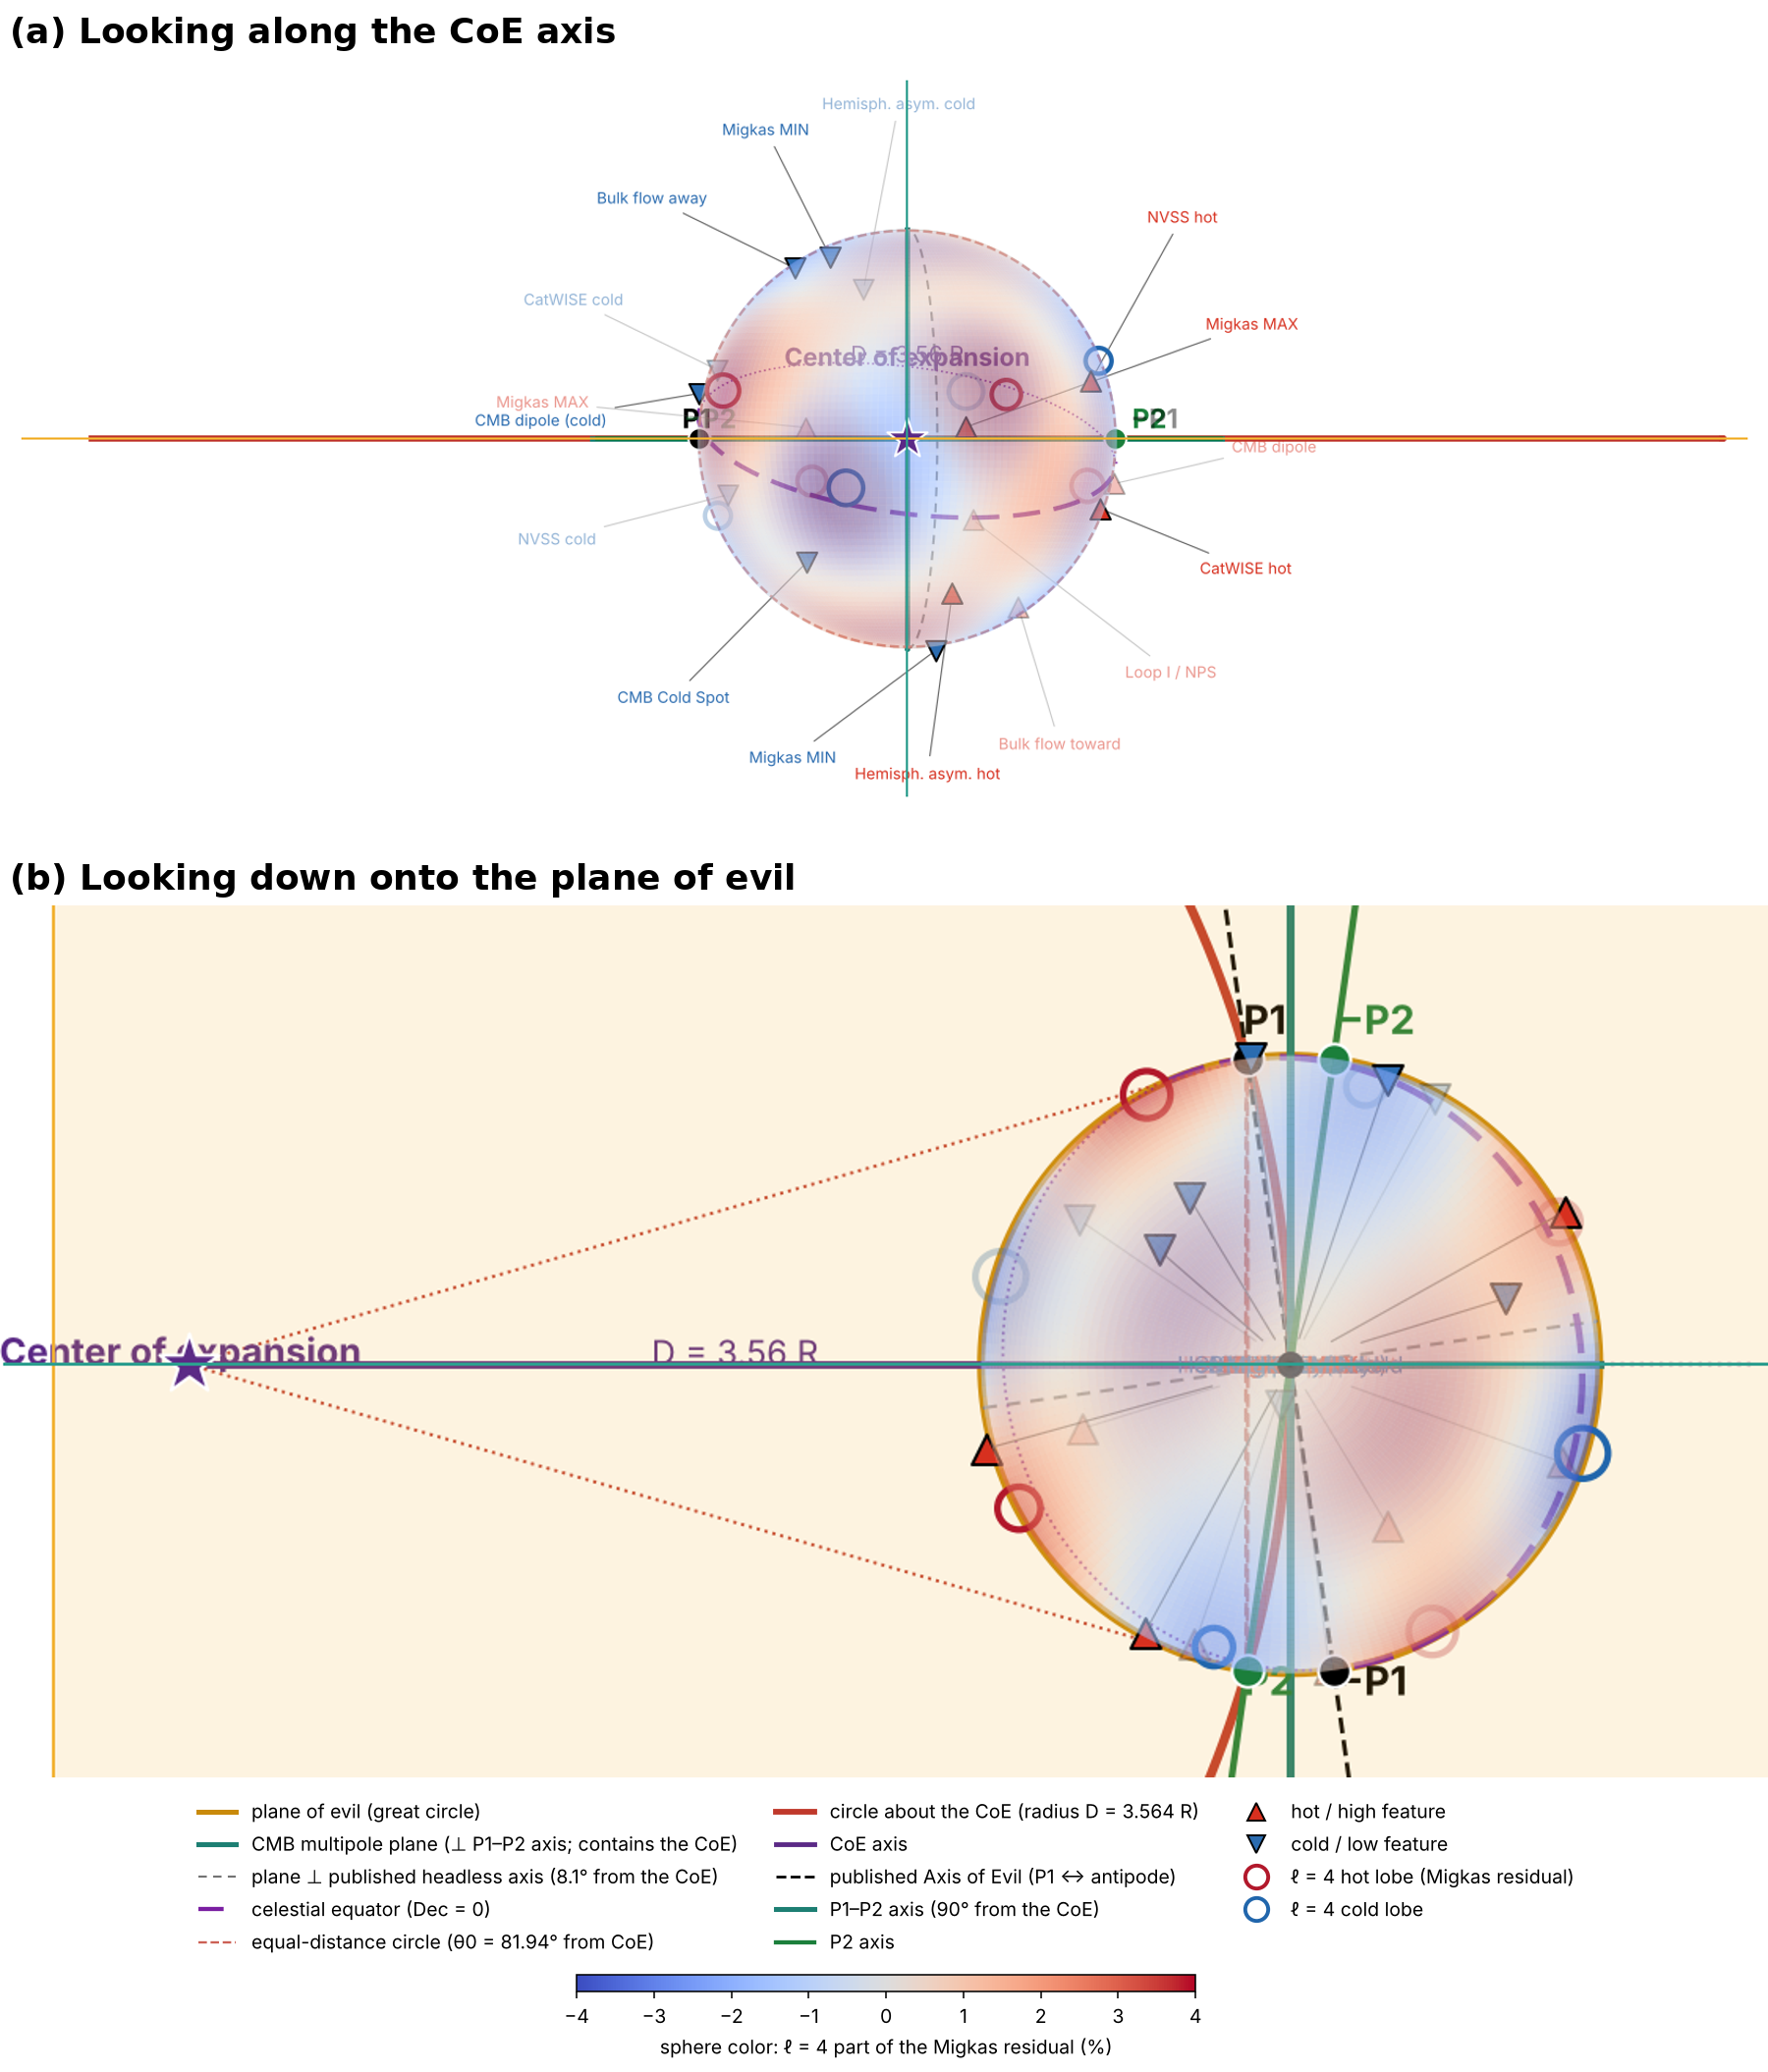
\includegraphics[width=0.88\textwidth]{figs/figA_frame_views_vertical.png}
\caption{The frame of Fig.~\ref{fig:frame} seen (a, top) along the CoE axis, with the CoE behind the observer at the center, and (b, bottom) from above the plane of evil. Symbols as in Fig.~\ref{fig:frame}.}\label{fig:views}
\end{figure}

\section{Low-$\ell$ axes in Planck SMICA}\label{app:smica}
Map: Planck PR3 SMICA temperature, smoothed to $3\dg$ FWHM, $N_{\rm side}=64$, monopole and dipole removed. Spherical harmonics up to $\ell=10$ were fitted by least squares to the unmasked pixels. For a trial axis $\hat n$, the statistic is $\sum_m m^2|a_{\ell m}|^2/\sum_m|a_{\ell m}|^2$ in a frame with $\hat n$ as pole \cite{LM05}, summed over $\ell=2,3$ for the combined axis; it was maximized over the sky. A mask at $|b|>30\dg$ leaves too little sky for a stable $\ell\le10$ fit and is not used. Code: \texttt{lowl.py}, \texttt{masked.py}.

\begin{table}[H]\centering\small
\caption{Quadrupole ($\ell=2$), octopole ($\ell=3$) and combined axes, and their relation to the frame. Distances between axes are headless.}\label{tab:smica}
\begin{tabular}{llcccc}\toprule
Sky & Multipoles & Axis $(l,b)$ & to P1--P2 axis & to published axis & CoE off plane\\\midrule
Full & $\ell=2$ & $(240.2\dg,+54.0\dg)$ & $4.3\dg$ & $12.3\dg$ & $4.2\dg$\\
 & $\ell=3$ & $(238.0\dg,+63.0\dg)$ & $7.2\dg$ & $10.9\dg$ & $0.1\dg$\\
 & $\ell=2,3$ & $(238.7\dg,+60.5\dg)$ & $5.1\dg$ & $10.5\dg$ & $1.3\dg$\\
$|b|>10\dg$ & $\ell=2$ & $(227.7\dg,+54.0\dg)$ & $10.6\dg$ & $18.4\dg$ & $9.9\dg$\\
 & $\ell=3$ & $(240.8\dg,+56.6\dg)$ & $2.7\dg$ & $10.6\dg$ & $2.5\dg$\\
 & $\ell=2,3$ & $(236.3\dg,+56.0\dg)$ & $5.3\dg$ & $13.1\dg$ & $4.9\dg$\\
$|b|>20\dg$ & $\ell=2$ & $(249.3\dg,+62.6\dg)$ & $5.9\dg$ & $5.7\dg$ & $4.2\dg$\\
 & $\ell=3$ & $(240.5\dg,+55.4\dg)$ & $3.3\dg$ & $11.3\dg$ & $3.3\dg$\\
 & $\ell=2,3$ & $(243.5\dg,+58.7\dg)$ & $2.2\dg$ & $8.5\dg$ & $0.2\dg$\\\bottomrule
\end{tabular}
\end{table}

The shift of the combined axis from the published axis points within $9$--$28\dg$ of the direction toward the P1--P2 axis, with size $8.5$--$13.1\dg$ against $8.1\dg$ predicted.

\begin{thebibliography}{99}\small\setlength{\itemsep}{0pt}\setlength{\parskip}{0pt}
\bibitem{Schwarz04} D.~J. Schwarz, G.~D. Starkman, D.~Huterer, C.~J. Copi, \emph{Phys.\ Rev.\ Lett.} \textbf{93}, 221301 (2004), astro-ph/0403353.
\bibitem{Copi07} C.~J. Copi, D.~Huterer, D.~J. Schwarz, G.~D. Starkman, \emph{Phys.\ Rev.\ D} \textbf{75}, 023507 (2007), astro-ph/0605135.
\bibitem{LM05} K.~Land, J.~Magueijo, \emph{Phys.\ Rev.\ Lett.} \textbf{95}, 071301 (2005), astro-ph/0502237.
\bibitem{RS07} A.~Raki\'c, D.~J. Schwarz, ``Correlating anomalies of the microwave sky: The Good, the Evil and the Axis'', astro-ph/0703266 (2007).
\bibitem{Secrest21} N.~J. Secrest et al., \emph{Astrophys.\ J.\ Lett.} \textbf{908}, L51 (2021).
\bibitem{Migkas20} K.~Migkas et al., \emph{Astron.\ Astrophys.} \textbf{636}, A15 (2020).
\bibitem{Migkas21} K.~Migkas et al., \emph{Astron.\ Astrophys.} \textbf{649}, A151 (2021).
\bibitem{Scolnic22} D.~Scolnic et al., \emph{Astrophys.\ J.} \textbf{938}, 113 (2022).
\bibitem{Jaffe05} T.~R. Jaffe, A.~J. Banday, H.~K. Eriksen, K.~M. G\'orski, F.~K. Hansen, \emph{Astrophys.\ J.\ Lett.} \textbf{629}, L1 (2005), astro-ph/0503213.
\bibitem{Jaffe06} T.~R. Jaffe et al., ``Bianchi type VII$_h$ models and the WMAP 3-year data'', astro-ph/0606046 (2006).
\bibitem{ST03} J.~Smoller, B.~Temple, ``Shock-wave cosmology inside a black hole'', \emph{Proc.\ Natl.\ Acad.\ Sci.\ USA} \textbf{100}, 11216 (2003), astro-ph/0210105.
\bibitem{ST09} J.~Smoller, B.~Temple, ``Expanding wave solutions of the Einstein equations that induce an anomalous acceleration into the Standard Model of Cosmology'', \emph{Proc.\ Natl.\ Acad.\ Sci.\ USA} \textbf{106}, 14213 (2009), arXiv:0901.1639.
\bibitem{STV17} J.~Smoller, B.~Temple, Z.~Vogler, ``An instability of the Standard Model of Cosmology creates the anomalous acceleration without dark energy'', \emph{Proc.\ R.\ Soc.\ A} \textbf{473}, 20160887 (2017), arXiv:1412.4001.
\bibitem{Planck18IV} Planck Collaboration, ``Planck 2018 results. IV. Diffuse component separation'', \emph{Astron.\ Astrophys.} \textbf{641}, A4 (2020).
\bibitem{Planck13XXVI} Planck Collaboration, ``Planck 2013 results. XXVI. Background geometry and topology of the Universe'', \emph{Astron.\ Astrophys.} \textbf{571}, A26 (2014).
\bibitem{Alnes06} H.~Alnes, M.~Amarzguioui, \emph{Phys.\ Rev.\ D} \textbf{74}, 103520 (2006).
\bibitem{Erickcek08} A.~L. Erickcek, M.~Kamionkowski, S.~M. Carroll, \emph{Phys.\ Rev.\ D} \textbf{78}, 123520 (2008).
\bibitem{He25} K.~He, K.~Migkas et al., FLAMINGO simulations of cluster scaling-relation anisotropy, arXiv:2504.01745 (2025).
\bibitem{Bao23} J.-B. Bao, N.~P. Bao, ``The Center and Spin of the Universe'', Preprints.org 202306.1689 (2023), not peer-reviewed.
\end{thebibliography}
\end{document}
